\documentclass[conference]{IEEEtran} % Camera-ready format

\usepackage{graphicx}             % import, scale, and rotate graphics
\usepackage{subfigure}            % group figures
\usepackage{url}                  % facilitate linebreaking of URLs
\usepackage[latin1]{inputenc}     % use characters with accents in the source
\usepackage{nicefrac}             % write fractions in the text
\usepackage{indentfirst}          % indent the first paragraph
\usepackage[super, negative]{nth}
\usepackage{multirow}
\usepackage{moreverb}
\usepackage{amsmath}
\usepackage{amssymb}
\usepackage{amsfonts}
\usepackage{dcolumn}
\usepackage[dvipsnames,usenames]{color}
\usepackage{xspace}


\usepackage{array,booktabs}
\usepackage{latexsym}
\usepackage{pifont}
\usepackage{colortbl}
\usepackage{bytefield}

\newcommand{\ed}[1]{\textsf{\textbf{[#1]}}}  %editorial comments
\newcommand{\dfn}[1]{\textit{#1}}            %introducing new terms
\newcommand{\revision}[1]{\tr{#1}}
\newcommand{\co}[2]{#1 & \tiny{$\pm#2$}}     %intervalles de confiance
\newcommand{\ttlexceeded}{\texttt{time-exceeded}\xspace}
\newcommand{\tpropagate}{\texttt{ttl-propagate}\xspace}
\newcommand{\echoreply}{\texttt{echo-reply}\xspace}
\newcommand{\echorequest}{\texttt{echo-request}\xspace}
\newcommand{\dstunreach}{\texttt{destination-unreachable}\xspace}
\newcommand{\traceroute}{\texttt{traceroute}\xspace}
\newcommand{\ping}{\texttt{ping}\xspace}
\newcommand{\scamper}{\texttt{scamper}\xspace}
\newcommand{\magallanes}{\textsc{Magallanes}\xspace}

\hyphenation{trace-route trace-routes trace-rout-ing}
\hyphenation{destination-un-reachable dest-ination-unreachable
destination-un-reach-able des-tination-unreachable desti-nation-unreachable
destina-tion-unreachable}
\hyphenation{AS-es}
\hyphenation{Topo-logy}

\graphicspath{{.}{./Figures/}}

\begin{document}

\title{	Unveiling the MPLS structure on Internet Topology} %Please, any suggestions is welcome
\author{Gabriel Davila Revelo{$^{\dag}$}, Mauricio Anderson Ricci{$^{\dag}$} , Benoit Donnet{$^{\ast}$},
Jos\'e Ignacio Alvarez-Hamelin{$^{\dag\ddag}$}\\
$\dag$ INTECIN, Facultad de Ingenier\'{\i}a, Universidad de Buenos Aires -- Argentina\\ 
\{gdavila, anderson, ihameli\}@cnet.fi.uba.ar, $\ddag$ CONICET -- Argentina \\
$\ast$ Universit\'e de Li\`ege, Li\`ege -- Belgium,~ 
benoit.donnet@ulg.ac.be\\
}

\maketitle

\begin{abstract}
toto
\end{abstract}

\section{Introduction}\label{intro}
% %%%%%%%%%%%%%%%%%%%%%
Internet topology refers to the study of the various types of
connectivity structures and representations between directly connected nodes on
the Internet architecture~\cite{Calvert97}. This representation aims at
obtaining models that represent  Internet with the greatest possible accuracy in order
to test new communications protocols, algorithms, QoS policies, traffic
engineering, etc.

The Internet topology can be seen at several abstraction levels i.e., IP
interface, router, subnetwork, PoP, and Autonomous System (AS) levels. All these
models have been widely studied in the past~\cite{DONNET13} . However, the
current state of the art of Internet deployments involves a great number of
technologies impacting the Internet Topology.  And those technologies deserve a
deep study in order to include them in Internet topology models.  For instance, 
\dfn{Multiprotocol Label Switching} (MPLS)~\cite{rfc3031} has been recently the
focus of several studies~\cite{SOM11,DONNET13,Vanaubel15}.  It has been
demonstrated that MPLS is a mature technology widely deployed for (mainly) load
balancing reasons or traffic engineering purposes.  Although few studies have
partially questioned its impact on Internet topology~\cite{BRICE07,Flach2012}, the impact of MPLS deployment on the Internet architecture has not been
studied yet in deep. The importance to study new architectural details, structure and topological
features related with MPLS usage would help to know the way in
which the Internet Service Providers (ISPs) use their networks or apply their
policies for traffic engineering as well as to better understand the today's
Internet architecture more accurately. Our work provides a study around the
impact of MPLS deployments over Internet Topology. Principally, we focus on the
bias involved in MPLS tunnel detection and on the features that MPLS modifies over traditional networks maps such as router level topology. For our purpose, we mainly based on  $k$-core
decomposition method~\cite{batagelj2002}. In this way, it has been shown
previously that the $k$-core decomposition is a relevant tool to describe
Internet Topology ~\cite{Alvarez06k, Serrano06, Serrano06, Alvarez08k}.

This paper adds complementary information around MPLS
usage on Internet. First, we present a quantification of the biases involved on
implicit MPLS tunnel detection. Additionally, we provided some properties and
architectural details related with MPLS deployment on router level topology. We found
that routers are commonly connected to  MPLS
networks. Finally, we found that ASes seems to have different MPLS structure 
according the type of MPLS tunnel that prevails.


The remainder of this paper is organized as follows: Sec.~\ref{related} provides
the state of the art and the background related to MPLS tunnels discovery. In
particular, it describes how MPLS tunnels can be revealed through active
measurements;  Sec.~\ref{dataset} explains how we collected data for this work;
Sec.~\ref{validation} presents our results related to \textit{mpls signatures}
accuracy; Sec.~\ref{cluster} presents the main contributions of this paper with
a detailed study around the behaviour of MPLS networks on the Internet Topology
and architectural details of some ASes with most MPLS usage; Finally,
Sec.~\ref{ccl} concludes this paper by summarizing its main achievements.


\section{Related Work}\label{related}
% %%%%%%%%%%%%%%%%%%%%
In this section, we first provide an overview of MPLS
(Sec.~\ref{related.overview}) before explaining how MPLS tunnels can be revealed
through active measurements (Sec.~\ref{related.revealing}).  We also position
this work regarding the state of the art.

\subsection{MPLS Overview}\label{related.overview}
%%%%%%%%%%%%%%%%%%%%%%%%%%%
The \dfn{Multiprotocol Label Switching} (MPLS)~\cite{rfc3031} was originally
designed to speed up the forwarding process. In practice, this was done with one
or more 32 bits \dfn{label stack entries} (LSE) inserted between the frame
header (Data-link layer) and the IP packet (Network layer).\footnote{MPLS is IP
layer protocol independent.} A given packet can manage several LSEs at the same
time. In this case, the packet is said having a \dfn{stack of labels}.  Each LSE
is made of four fields:  a 20-bit label value used for forwarding the packet to
the next router, a 3-bit Traffic Class field for quality of service (QoS),
priority, and Explicit Congestion Notification (ECN)~\cite{rfc5462}, a 1-bit
bottom of stack flag (when set the current label is the last in the
stack~\cite{rfc3032}), and an 8-bit time-to-live (LSE-TTL) field having the same
purpose as the IP-TTL field~\cite{rfc3443}.

MPLS routers, called \dfn{Label Switching Routers} (LSRs), exchange labelled
packets over \dfn{Label Switched Paths} (LSPs).   The first MPLS router
(\dfn{Ingress Label Edge Router}, or Ingress LER, i.e., the tunnel entry point)
adds the label stack, while the last MPLS router (\dfn{Egress Label Edge
Router}, or Egress LER, i.e., the tunnel exit point) removes the label stack.
In some cases, for performance reasons, the LSE stack may be removed by the
penultimate MPLS router (\dfn{penultimate hop popping}, PHP).  The Egress LER
then performs a classic IP lookup and forwards the traffic, reducing so the load
on the Egress LER (specially if the Egress LER is shared among several LSPs).
This means that, when using PHP, the tunnel exit is one hop before the Egress
LER. % In its most basic operation, LSPs are constructed along best effort routes
%using the \dfn{Label Distribution Protocol} (LDP~\cite{rfc5036}). More specific
%LSPs may be constructed for Traffic Engineering purposes, using an extension of
%the RSVP protocol, \dfn{RSVP-TE}~\cite{rfc3209}. In these two cases, the label
%stack contains only one LSE. A more complex usage is for Virtual Private Networks
%(VPN~\cite{rfc2917}), where LSPs are constructed using either LDP or RSVP-TE,
%and an additional LSE at the bottom of the label stack is used to specify a Virtual
%Routing Table at the Egress. In this case, the bottom of the stack is constant
%along an LSP, while the top of the stack is modified at each hop, as in the
%previous cases.

\subsection{Revealing MPLS Tunnels}\label{related.revealing}
% %%%%%%%%%%%%%%%%%%%%%%%%%%%%%%%%%%
MPLS routers may send ICMP \ttlexceeded messages when the LSE-TTL expires. In
order to debug networks where MPLS is deployed, routers may also implement
RFC4950~\cite{rfc4950}, an extension to ICMP allowing a router to embed an MPLS
LSE in an ICMP \ttlexceeded message. In that case, the router simply quotes the
MPLS LSE (or the LSE stack) of the received packet in the ICMP \ttlexceeded
message. RFC4950 is particularly useful for operators as it allows them to
verify the correctness of their MPLS tunnels and TE policy.

If the Ingress LER copies the IP-TTL value to the LSE-TTL field rather than
setting the LSE-TTL to an arbitrary value such as 255, LSRs along the LSP will
reveal themselves when using traceroute via ICMP messages even if they do not
implement RFC4950. Operators can configure this action using the \tpropagate
option provided by the router manufacturer~\cite{rfc3443} (while, to the best of
our knowledge, the RFC4950 is just a matter of implementation and cannot be
deactivated on recent routers supporting it). 

Using those two features, Sommers et al.~\cite{SOM11} provide an extensive study
of MPLS tunnels as observed in CAIDA's topology data.  In this data, they find
tunnels in 7\% of ASes, and the fraction is constant over the years of data
considered.  In addition, Sommers et al. propose a statistical methodology to
infer MPLS tunnels in archived data where ICMP extensions are not recorded.
Vanaubel et al.~\cite{Vanaubel15} propose a classification of path diversity
according to MPLS deployment.  Their classification reveals the actual usage of
MPLS (e.g., load balancing, traffic engineering) according to the inferred label
distribution protocol.  Finally, it has also been demonstrated that MPLS tunnels
may have an impact on Internet topology discovery tools.  For instance, the
presence of MPLS tunnels may interfere with load balancing
detection~\cite{BRICE07} or violate the destination-based
forwarding~\cite{Flach2012}.

Donnet et al.~\cite{Donnet12} propose a taxonomy of MPLS tunnels based on how
they react to \traceroute probes according to their compliance (or not) to
RFC4950 for MPLS and the \tpropagate option.  The classes proposed are:
\dfn{explicit tunnels} (i.e., \tpropagate and RFC4950 are enabled),
\dfn{implicit tunnels} (i.e., the router that pushes the MPLS label enables the
\tpropagate option but LSRs do not implement RFC4950), \dfn{opaque tunnels}
(i.e., the LH implements RFC4950 but the ingress LER does not enable the
\tpropagate option), and, finally, \dfn{invisible tunnels} (i.e., the ingress
LER does not enable the \tpropagate option and RFC4950 is not implemented by the
LH router).  Implicit and opaque tunnels can be revelead as follows:
\begin{enumerate}
  \item a quoted IP-TTL (\dfn{qTTL}) in ICMP \ttlexceeded messages $>1$ will
  likely reveal the \tpropagate option at the ingress LER of an LSP. For each
  subsequent \traceroute probe within an LSP, the qTTL will be one greater
  resulting in an increasing sequence of qTTL values in \traceroute.  This is
  illustrated in Fig.~\ref{validation.qTTLFig};
  \item  \#hops differences with the IP-TTL in \echoreply messages
  (\dfn{u-turn}).  It relies on the fact that LSRs along an LSP present an
  \textit{original label stack} default routing behavior: when the LSE-TTL
  expires, an LSR first sends the \ttlexceeded reply to the Egress LER which
  then forwards the reply on its own to the probing source, while an LSR
  replies to other probes using its own IP routing table if available. Summarizing, 
  $\textit{u-turn}=\text{TTL}_{\text{echo-reply}}-\text{TTL}_{\text{time-exceeded}}$.
  The expected u-turn value is in the form $[2L, 2L-2, 2L-4,..., 2]$ where $L$
  is the tunnel length and the array position corresponds to the LSR position
  within the LSP.
  \item opaque tunnels are revealed through an \textit{abnormal} LSE-TTL
  ($1<$LSE-TTL$<255$) returned by the LH in the \ttlexceeded reply.
\end{enumerate}

Additional study by Vanaubel et al.~\cite{VAN2013} shows that the probing
heuristic to detect implicit tunnels seems quite reliable.  However, u-turn
signatures are by definition more subject to false positives than qTTL ones. 
This is exactly what we tackle in this paper (and, consequently, our work is
complementary to Vanaubel et al.~\cite{VAN2013}): we want to test u-turn
signature accuracy.

%Figura u-turn
% \begin{figure*}[!t]
%   \begin{center}
%     \subfloat[Tunnel Length Distribution]{\label{hist_length}
%       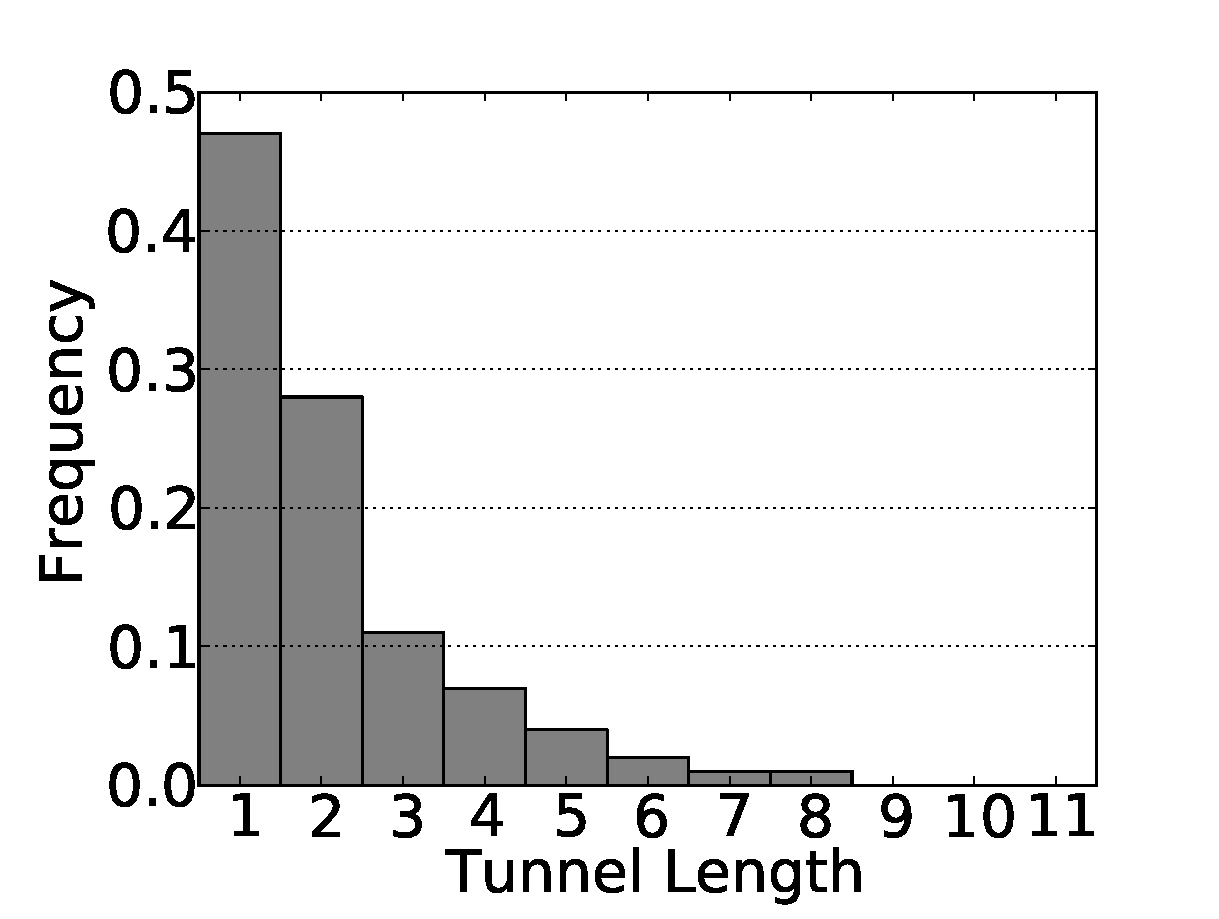
\includegraphics[width=6cm]{hist_length}}
%       \hfil
%     \subfloat[\textit{qTTL} and $n$-position comparison]{\label{n_vs_qttl}
%       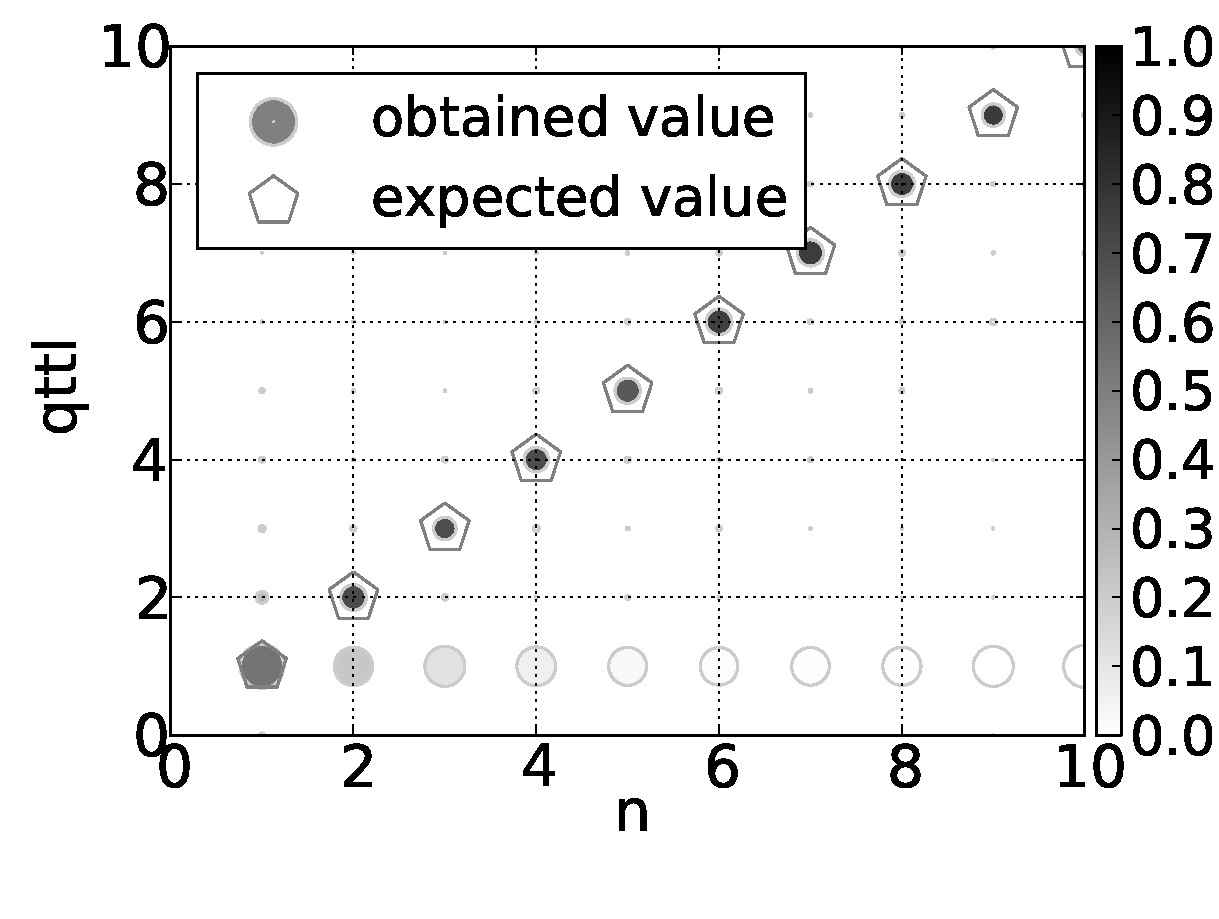
\includegraphics[width=6cm]{n_vs_qttl}} 
%       \hfil
%     \subfloat[\textit{u-turn} on LSRs revealed through RFC4950 and \textit{qTTL}]{\label{fig_uturn_a}
%       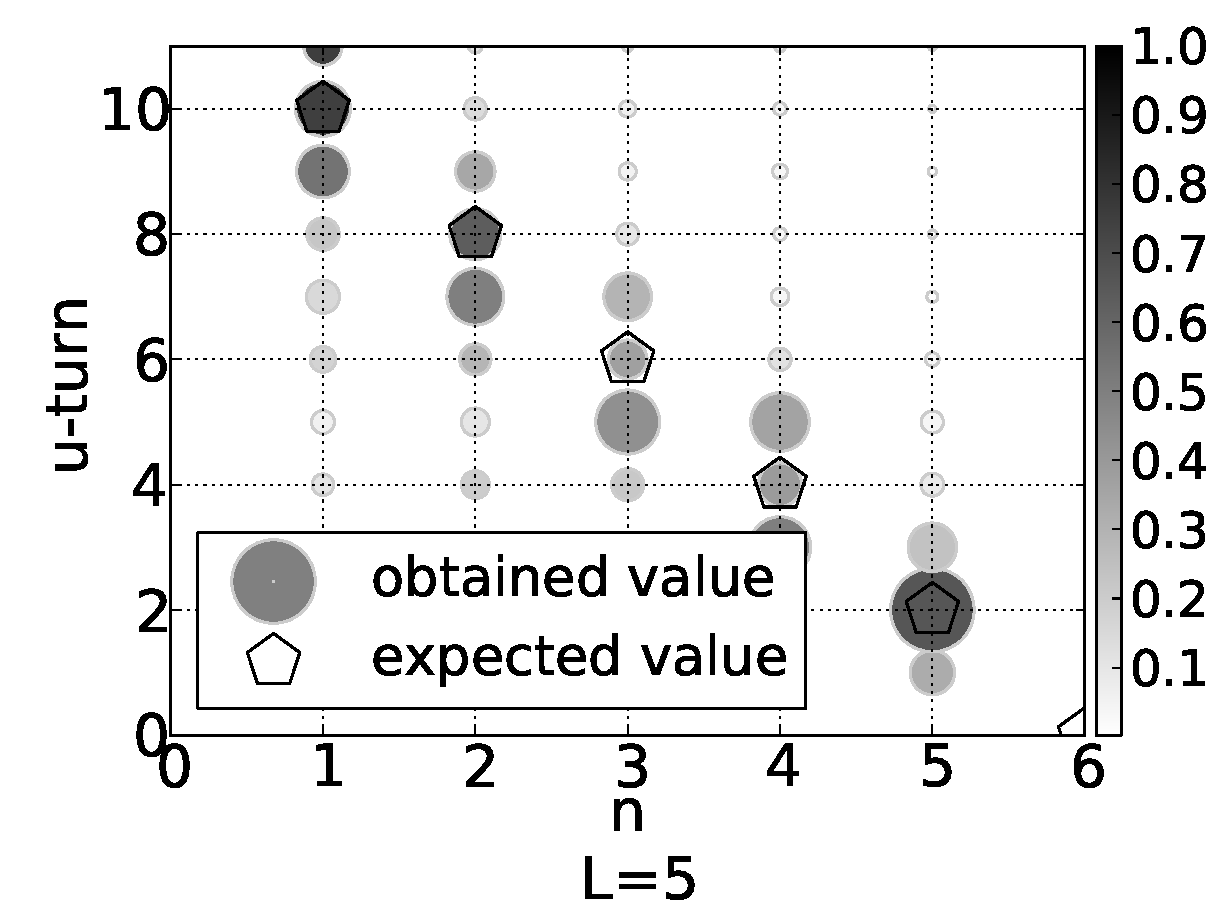
\includegraphics[width=6cm]{n_vs_uturn_L5_exp}}
%       \hfil
%     \subfloat[\textit{u-turn} on LSRs where no other signature was found]{\label{fig_uturn_b}
%       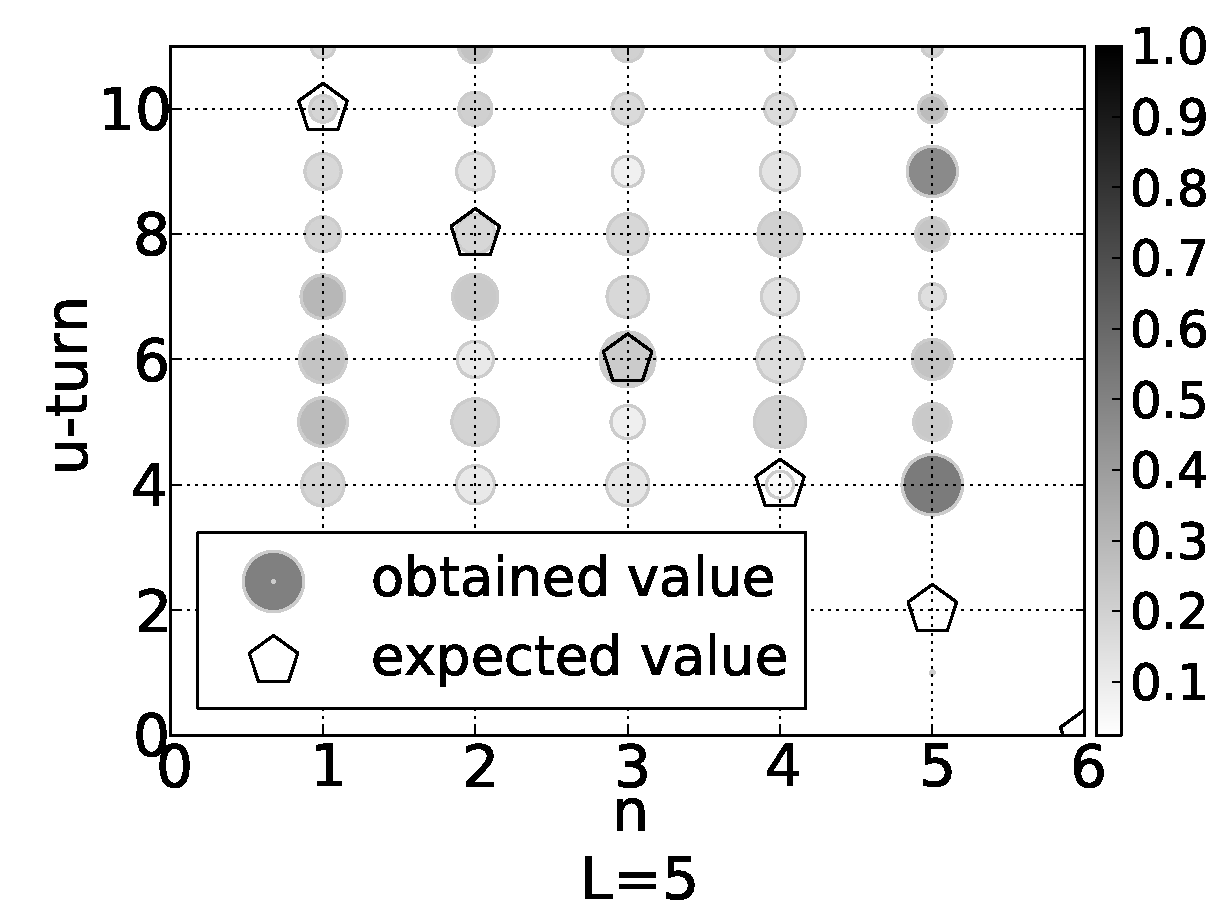
\includegraphics[width=6cm]{n_vs_uturn_L5}}
%    \end{center}
%   \caption{ Comparison between obtained and expected values for \textit{qTTL} and
%   \textit{u-turn} signatures. On figures (b), (c) and (d) the circle size in the scatter plot is related with the occurrence frequency of \textit{y-axis} values regarding each $n$-position. The
%   transparency of the circle is related with occurrence frequency of $n$-position  regarding each \textit{y-axis} value, e.g., on figure (b) for values where $n>1$, the biggest circles are mainly located on  $\textit{qTTL}=1$ and $\textit{qTTL}=n$ so this suggest that for a given $n$-position the \textit{qTTL} value usually takes either the value of $1$ or $n$; in the same way, the transparency value suggests that for a given \textit{qTTL} value the $n$-position usually takes the same \textit{qTTL} value.  \textbf{Figure (c)} and \textbf{Figure (d)} suggest that \textit{u-turn} value is overestimated. }
%   \label{ig_signatures}
% \end{figure*}

% \section{Related Work}\label{related}
% %%%%%%%%%%%%%%%%%%%%
% In the last years, MPLS~\cite{rfc3031} has been more and more investigated by
% the researchers.  This works mainly focused on MPLS tunnels detection. For
% instance, \Sommers et al.~\cite{SOM11} studied the MPLS deployment that is
% explicitly revealed through \textit{RFC 4950} extension. They also
% proposed a methodology to infer MPLS tunnels in archived data where ICMP extensions are not
% recorded. Most recently Donnet et al.~\cite{Donnet12} provided a
% taxonomy for MPLS tunnels and propose algorithms for detecting MPLS tunnels
% depending on the way that the LSRs react to the \textit{ttl-propagate} and
% \textit{RFC 4950} options. \ed{BD: I would remove this paragraph as it
% introduces concepts (RFC4950, LSRs, \ldots) that have not been }
% 
% It has also been studied the path diversity related with MPLS deployments. In
% this way, \textit{Vanaubel et al.} \cite{Vanaubel15} recently proposed and
% algorithm to better understand the path diversity and their usage within a given
% AS.
% 
% In this way, our work is complementary to tunnel detection issues. We test
% carefully some of the ways that reveals  MPLS tunnels and provided an analysis
% of how the MPLS tunnels impact the Internet Topology structure.

% \subsection{MPLS overview}\label{related.mpls}
% % %%%%%%%%%%%%%%%%%%%%%%%%% 
% MPLS \cite{RFC3031} was originally designed
% to speed up the forwarding process. In practice, this was done with one or more
% 32 bits Label Stack Entries (LSE) inserted between the frame header  and the IP
% packet.
% 
% In a MPLS network, packets are forwarded using an exact match lookup of a 20-bit
% label found in the LSE. An MPLS LSE also has a Time-To-Live (TTL) called LSE-TTL
% field and a Type-of-Service (ToS) field \cite{rfc1771}. At each MPLS hop, the
% label of the incoming packet is replaced by a corresponding outgoing label found
% in an MPLS switching table. A portion of a path where the forwarding decision is
% not anymore based on longest prefix matching but rather on MPLS features is
% known as an MPLS tunnel. A router with label switching capabilities is called
% Label Switching Router (LSR). A series of LSRs connected together form a Label
% Switched Path (LSP). The first router where the incoming packet includes a LSE
% is called ingress Label Edge Router (LER) and the last router that \textit{pops}
% the LSE is called Last Hop (LH).

% \subsection{Revealing MPLS tunnels} \label{related.signatures}
% 
% \textit{Donnet et al.} \cite{Donnet12} provided a taxonomy for MPLS tunnels
% revealed by traceroute and developed algorithms in order to detect it based on
% the way that LSR react to \textit{ttl-propagate}  and \textit{RFC 4950} option.
% Basically, their proposes two kind of visible MPLS tunnels: explicit tunnels and
% implicit tunnels.
% 
% Explicit tunnels are based on \textit{RFC 4950} implementation. MPLS routers may
% send ICMP time-exceeded messages when the LSE-TTL expires. The \textit{RFC 4950}
% is an extension to ICMP allowing a router to embed an MPLS LSE in an ICMP
% time-exceeded message. In that case, when the LSE-TTL expires on a MPLS router,
% it simply quotes the MPLS label stack in the ICMP \textit{time-exceeded}
% message.
% 
% Implicit tunnels discovery are based on two signatures detection: \textit{qttl}
% and \textit{u-turn} signature. The \textit{qttl} signature is relate with
% \textit{ttl-propagate} option. If  \textit{ttl-propagate} is implemented the LER
% copies the IP-TTL value to the LSE-TTL field rather than setting the LSE-TTL to
% an arbitrary value such as 255. In this way, the LSRs along the LSP will reveal
% themselves via ICMP messages even if they do not implement \textit{RFC 4950},
% i.e., if $\textit{qttl}>1$  the ICMP message was generated by an interfaces that
% belongs to an MPLS tunnel. The \textit{u-turn} signature relies on the fact that
% most LSRs in an LSP present a common behaviour: when the LSE-TTL expires, the
% LSR sends the ICMP \textit{time-exceeded} message to the LH router which then
% forwards the reply to the probing source, while an LSR replies to other probes
% such as  ICMP \textit{echo} packets using directly its own IP routing table if
% available. The variation between these two TTLs values is called \textit{u-turn}
% signature, i.e.,
% $\textit{u-turn}=TTL_{\text{echo-reply}}-TTL_{\text{time-exceeded}}$.  The
% expected \textit{u-turn} value in the form $[2L, 2L-2, 2L-4,..., 2]$ where $L$
% is the tunnel length and the array position correspond to the LSR position
% within the tunnel.
% 
% The \textit{qttl} signature ($\textit{qttl}>1$) is present just in MPLS
% behaviour.
% Commonly there is not another way to get a $\textit{qttl}>1$. However,
% \textit{u-turn} signature could be caused for another Internet issues such as
% police routing or load balancing paths, that produces different lengths in the
% return path.

% In this paper we consider that \textit{RFC 4950} implementation and
% \textit{qttl} signature are highly reliable methods to reveal MPLS tunnels and
% we mainly focus on to test \textit{u-turn} signature accuracy.

% \subsection{Diversity on MPLS paths}
% 
% \textit{Vanaubel et al.} \cite{SOM11} proposed a classification of path
% diversity on MPLS deployments. Their algorithm allow to classify the kind of
% diversity path regarding the behaviour of mpls labels on explicit tunnels. The
% authors propose basically a path classification based on physical diversity
% i.e., paths with different IP interfaces; and logical diversity i.e., paths with
% the same IP interfaces but different labels. The work show a detailed study of
% path diversity over the top of ASs with most MPLS tunnels discovered.       

\section{Data Collection}\label{dataset}
% %%%%%%%%%%%%%%%%%%%%%%%
In order to get MPLS data, we develop a tool called
\magallanes\footnote{\magallanes is freely available at \url{\ldots}} allowing
us to easily run and manage \scamper~\cite{Luckie10} based probes through the
PlanetLab (PL) infrastructure.  \magallanes starts by randomly allocating
several vantage points (VP) within the available set of PL nodes.  It next
distribues, among those VPs, a given number of probe targets.
To achieve some geographical uniformity in target selection, \magallanes uses
data provived by IP geolocation database maxmind.\footnote{See
\url{www.maxmind.com}.  Although we know that IP geolocation databases suffer
from strong accuracy limits~\cite{geolocation}, we believe it is enough for our
purpose as we do not need accurate geolocation.}  In this way, it chooses the
targets randomly and proportionality distributed according to the number of
subnets assigned by the Regional Internet Registry (RIR) to each region.
Additionally, \magallanes allows one to store the experiments results on a
centralized database and to perfom alias resolution using MIDAR~\cite{Keys13}.

We ran \magallanes on October \nth{31}, 2015.  We chose 100 VPs and selected
10,000 targets per VP.  Each VP managed its own set of targets, meaning that
probes targets are disjoint sets between VPs.  \scamper was configured to run
ICMP Paris traceroute~\cite{BRICE06}.  To get the \textit{u-turn} signature,
we sent a \ping to each hop revealed by Paris traceroute. We sent six
ICMP \echorequest packets from the same VP.  Six ICMP \echoreply allow us to
infer with $95\%$ confidence if there is a single return path and, 
therefore, reduce measurement errors caused by a reverse path containing
load-balanced segments of different lengths~\cite{BRICE07}. 

As a result we discovered around 270,000 IP interfaces,  520,000 links, $42\%$
of which were available to run MIDAR and we found aliases successfully on $19\%$
of then. To match IP interfaces to ASes, we used the CAIDA
dataset~\cite{caida_ref} derived from Routeviews \footnote{See
\url{www.routeviews.org}} and collected the same day as the exploration.
Additionally, we found that $44\%$ of traces collected traverse at least one
MPLS tunnel.  The amount of explicit tunnels is highly superior to implicit
ones. We discovered explicit tunnels on $34\%$ of traceroutes and at least one
implicit tunnel on $16\%$. Surprisingly, we found more implicit tunnels revealed
through \textit{u-turn} signature ($12\%$) rather than \textit{qTTL} signature
($4\%$). However, the \textit{qTTL} signature matched with at least $63\%$ of
the explicit tunnels. We discuss these results in the next sections. Finally, we
did not found opaque tunnels, confirming so their rarity~\cite{VAN2013}.

\section{MPLS Signatures Validation}\label{validation}
% %%%%%%%%%%%%%%%%%%%%%%%%%%%%%%%%%%%%

\begin{figure}[!t]
  \begin{center}
    \subfigure[Example of qTTL signature for an implicit MPLS tunnel.]{\label{validation.qTTLFig}
      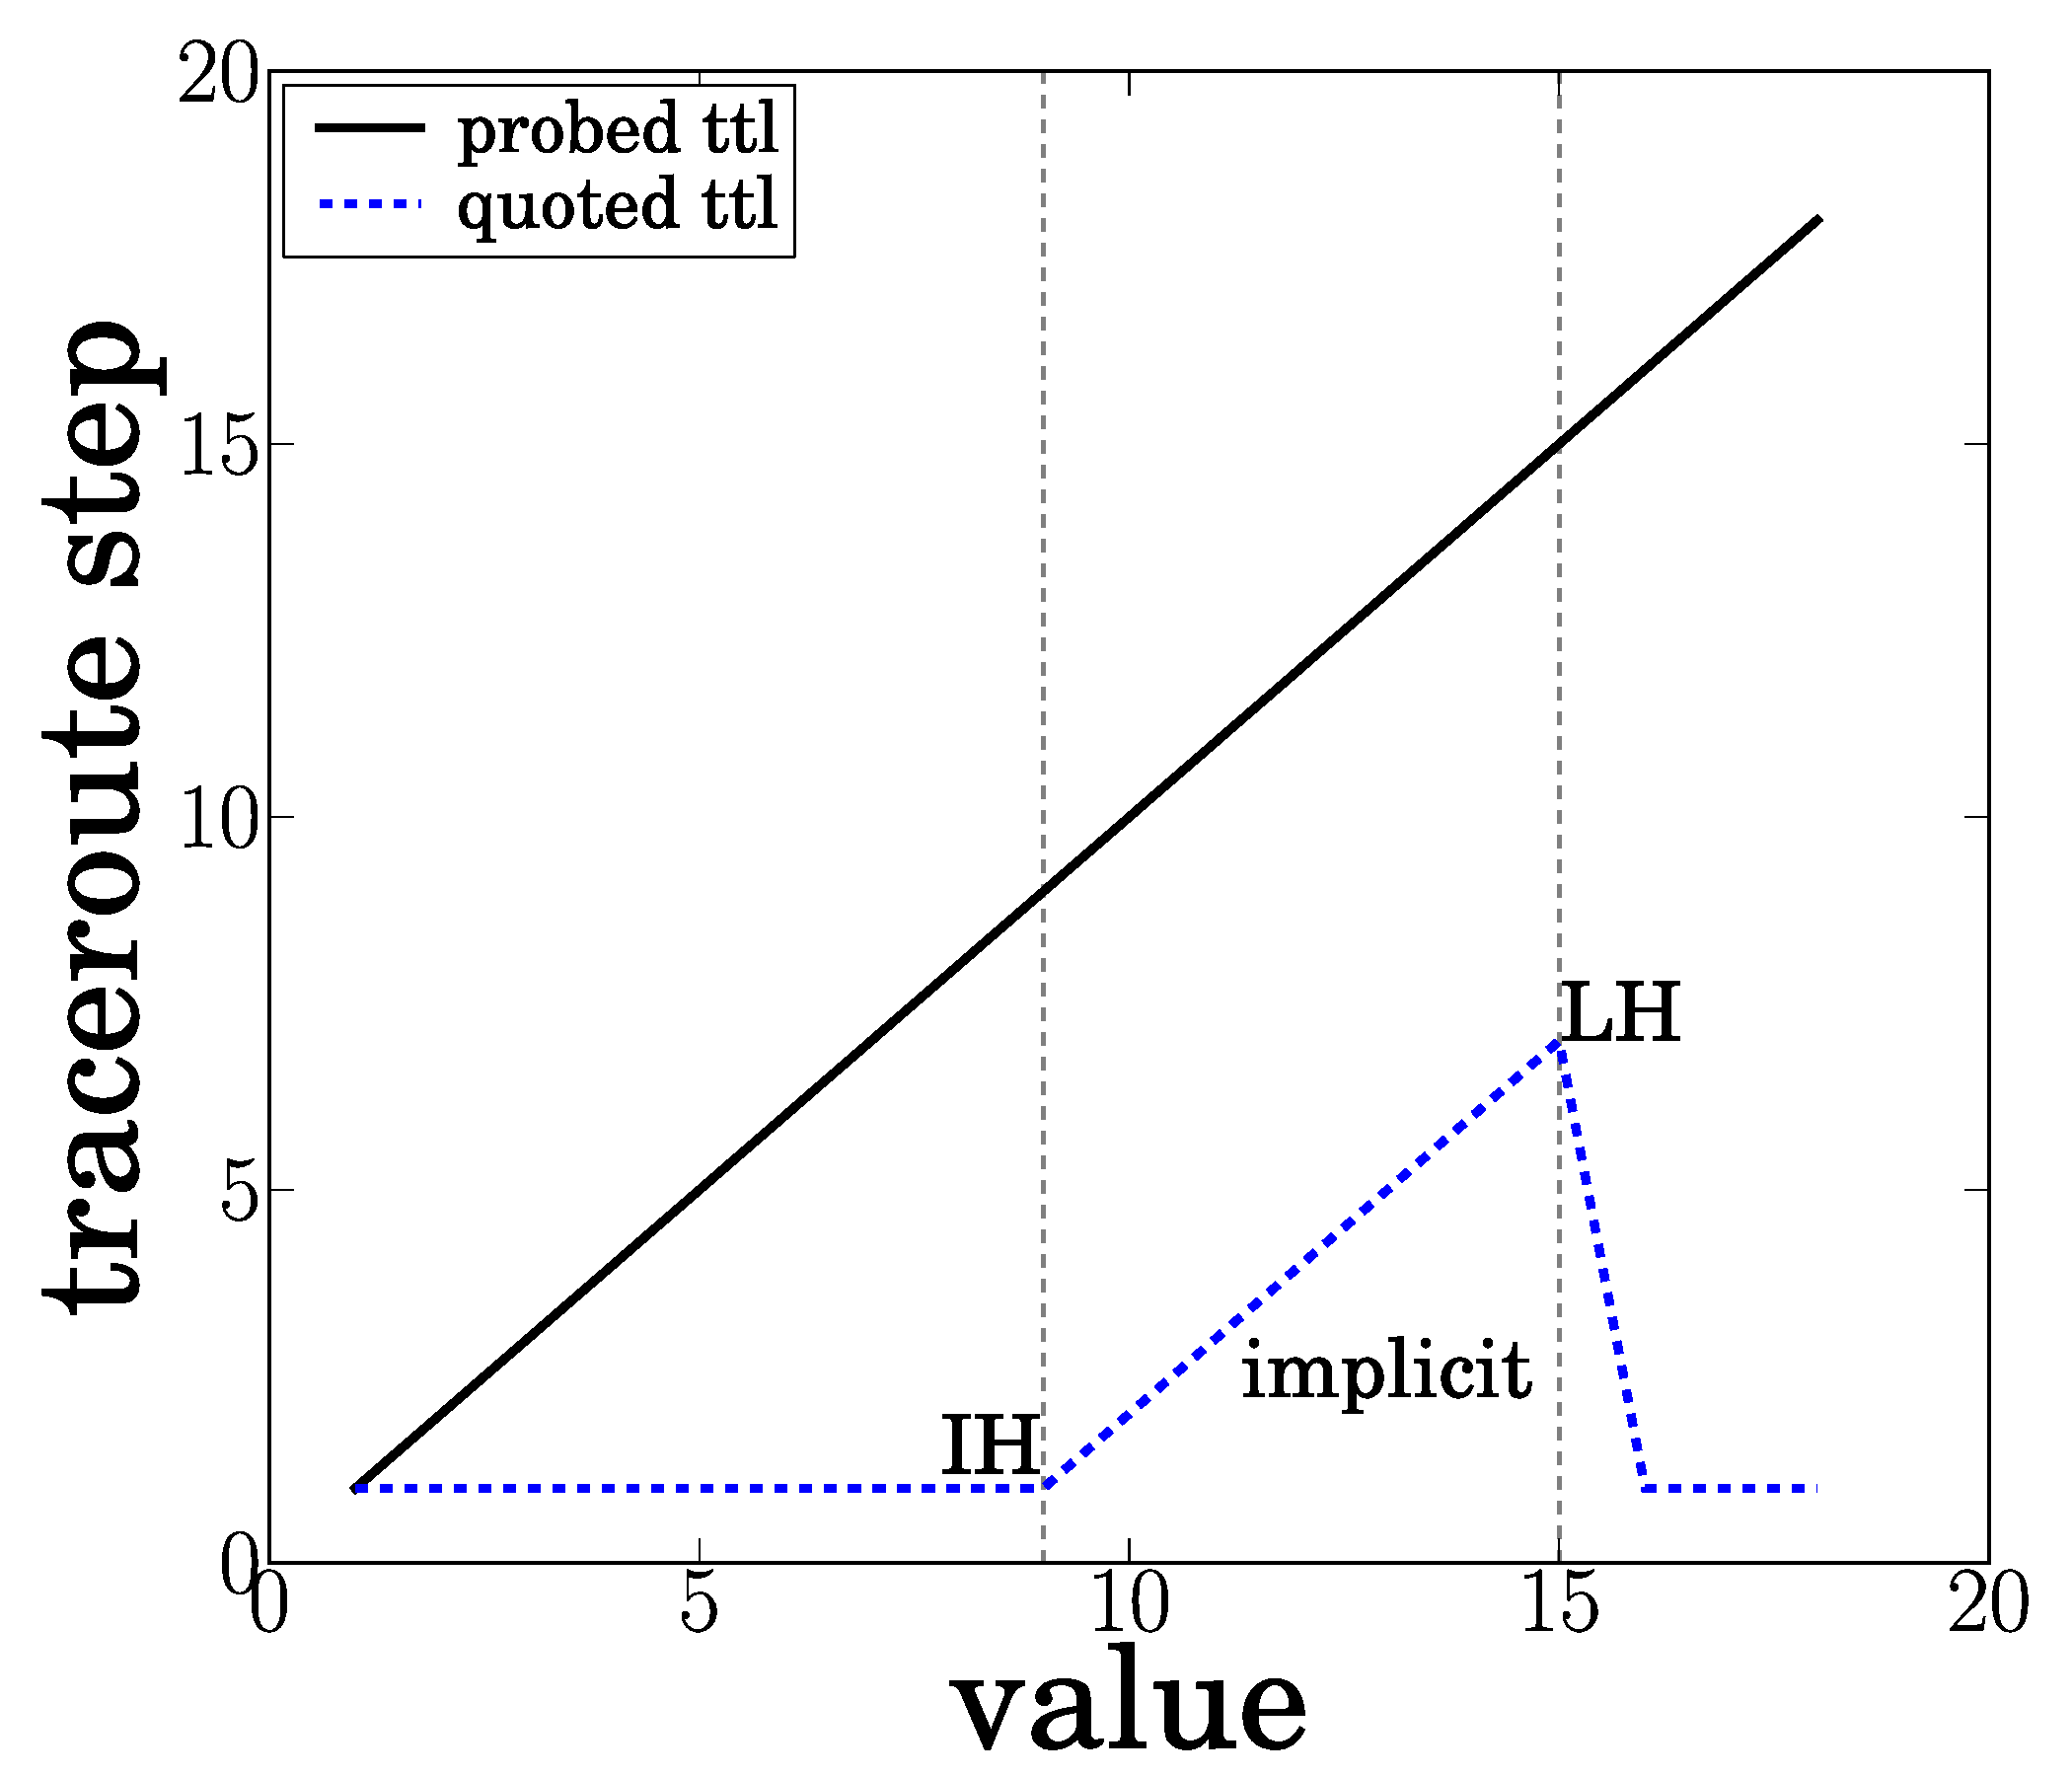
\includegraphics[width=4cm]{QuotedTTL}}
\hspace{-0.3cm}      
    \subfigure[Example of u-turn signature for an implicit MPLS tunnel]{\label{validation.uturn1Fig}
      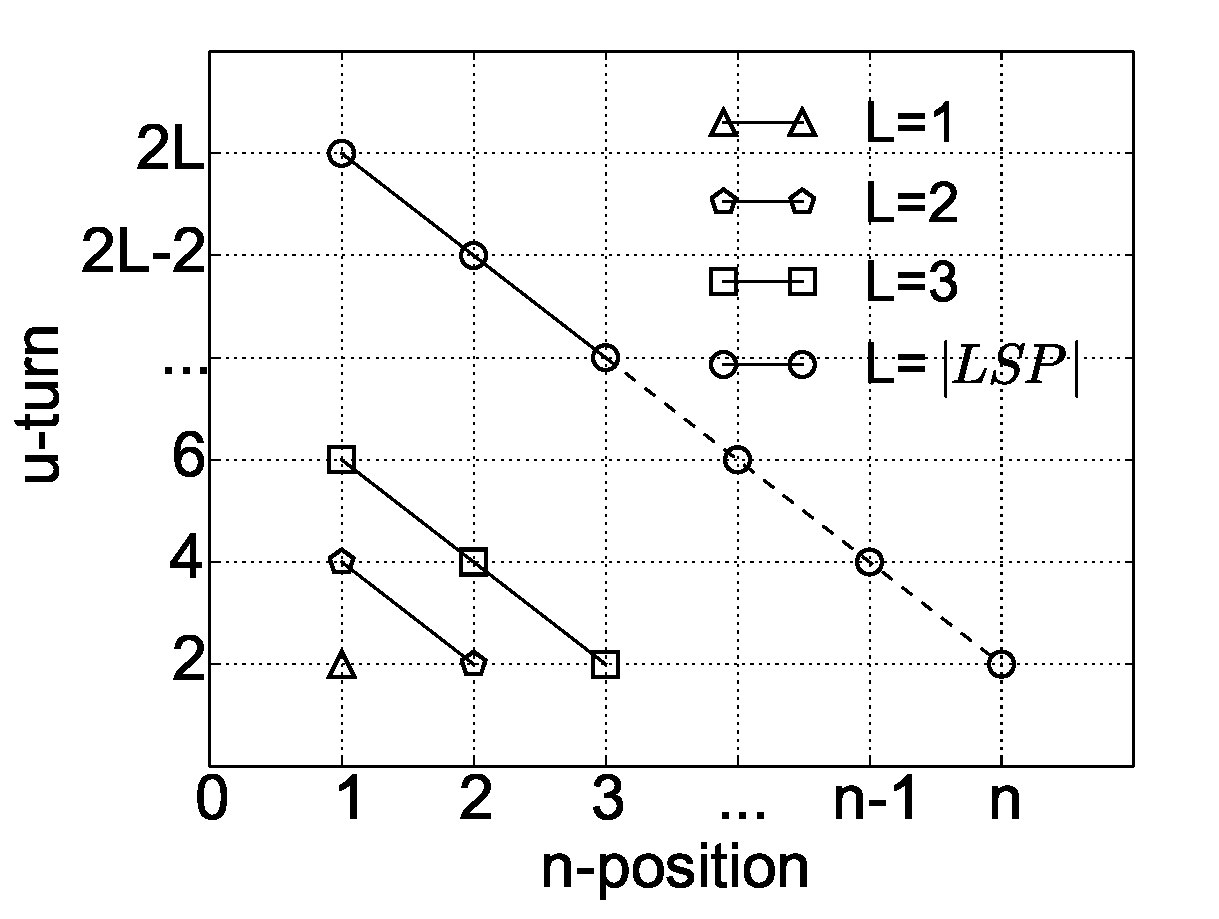
\includegraphics[width=4.5cm]{uturn1}}  
  \end{center}
  \caption{Signatures behaviour for implicit MPLS tunnels.}
  \label{validation.signatures.fig}
\end{figure}



%\begin{figure}[!t]
%  \begin{center}
%    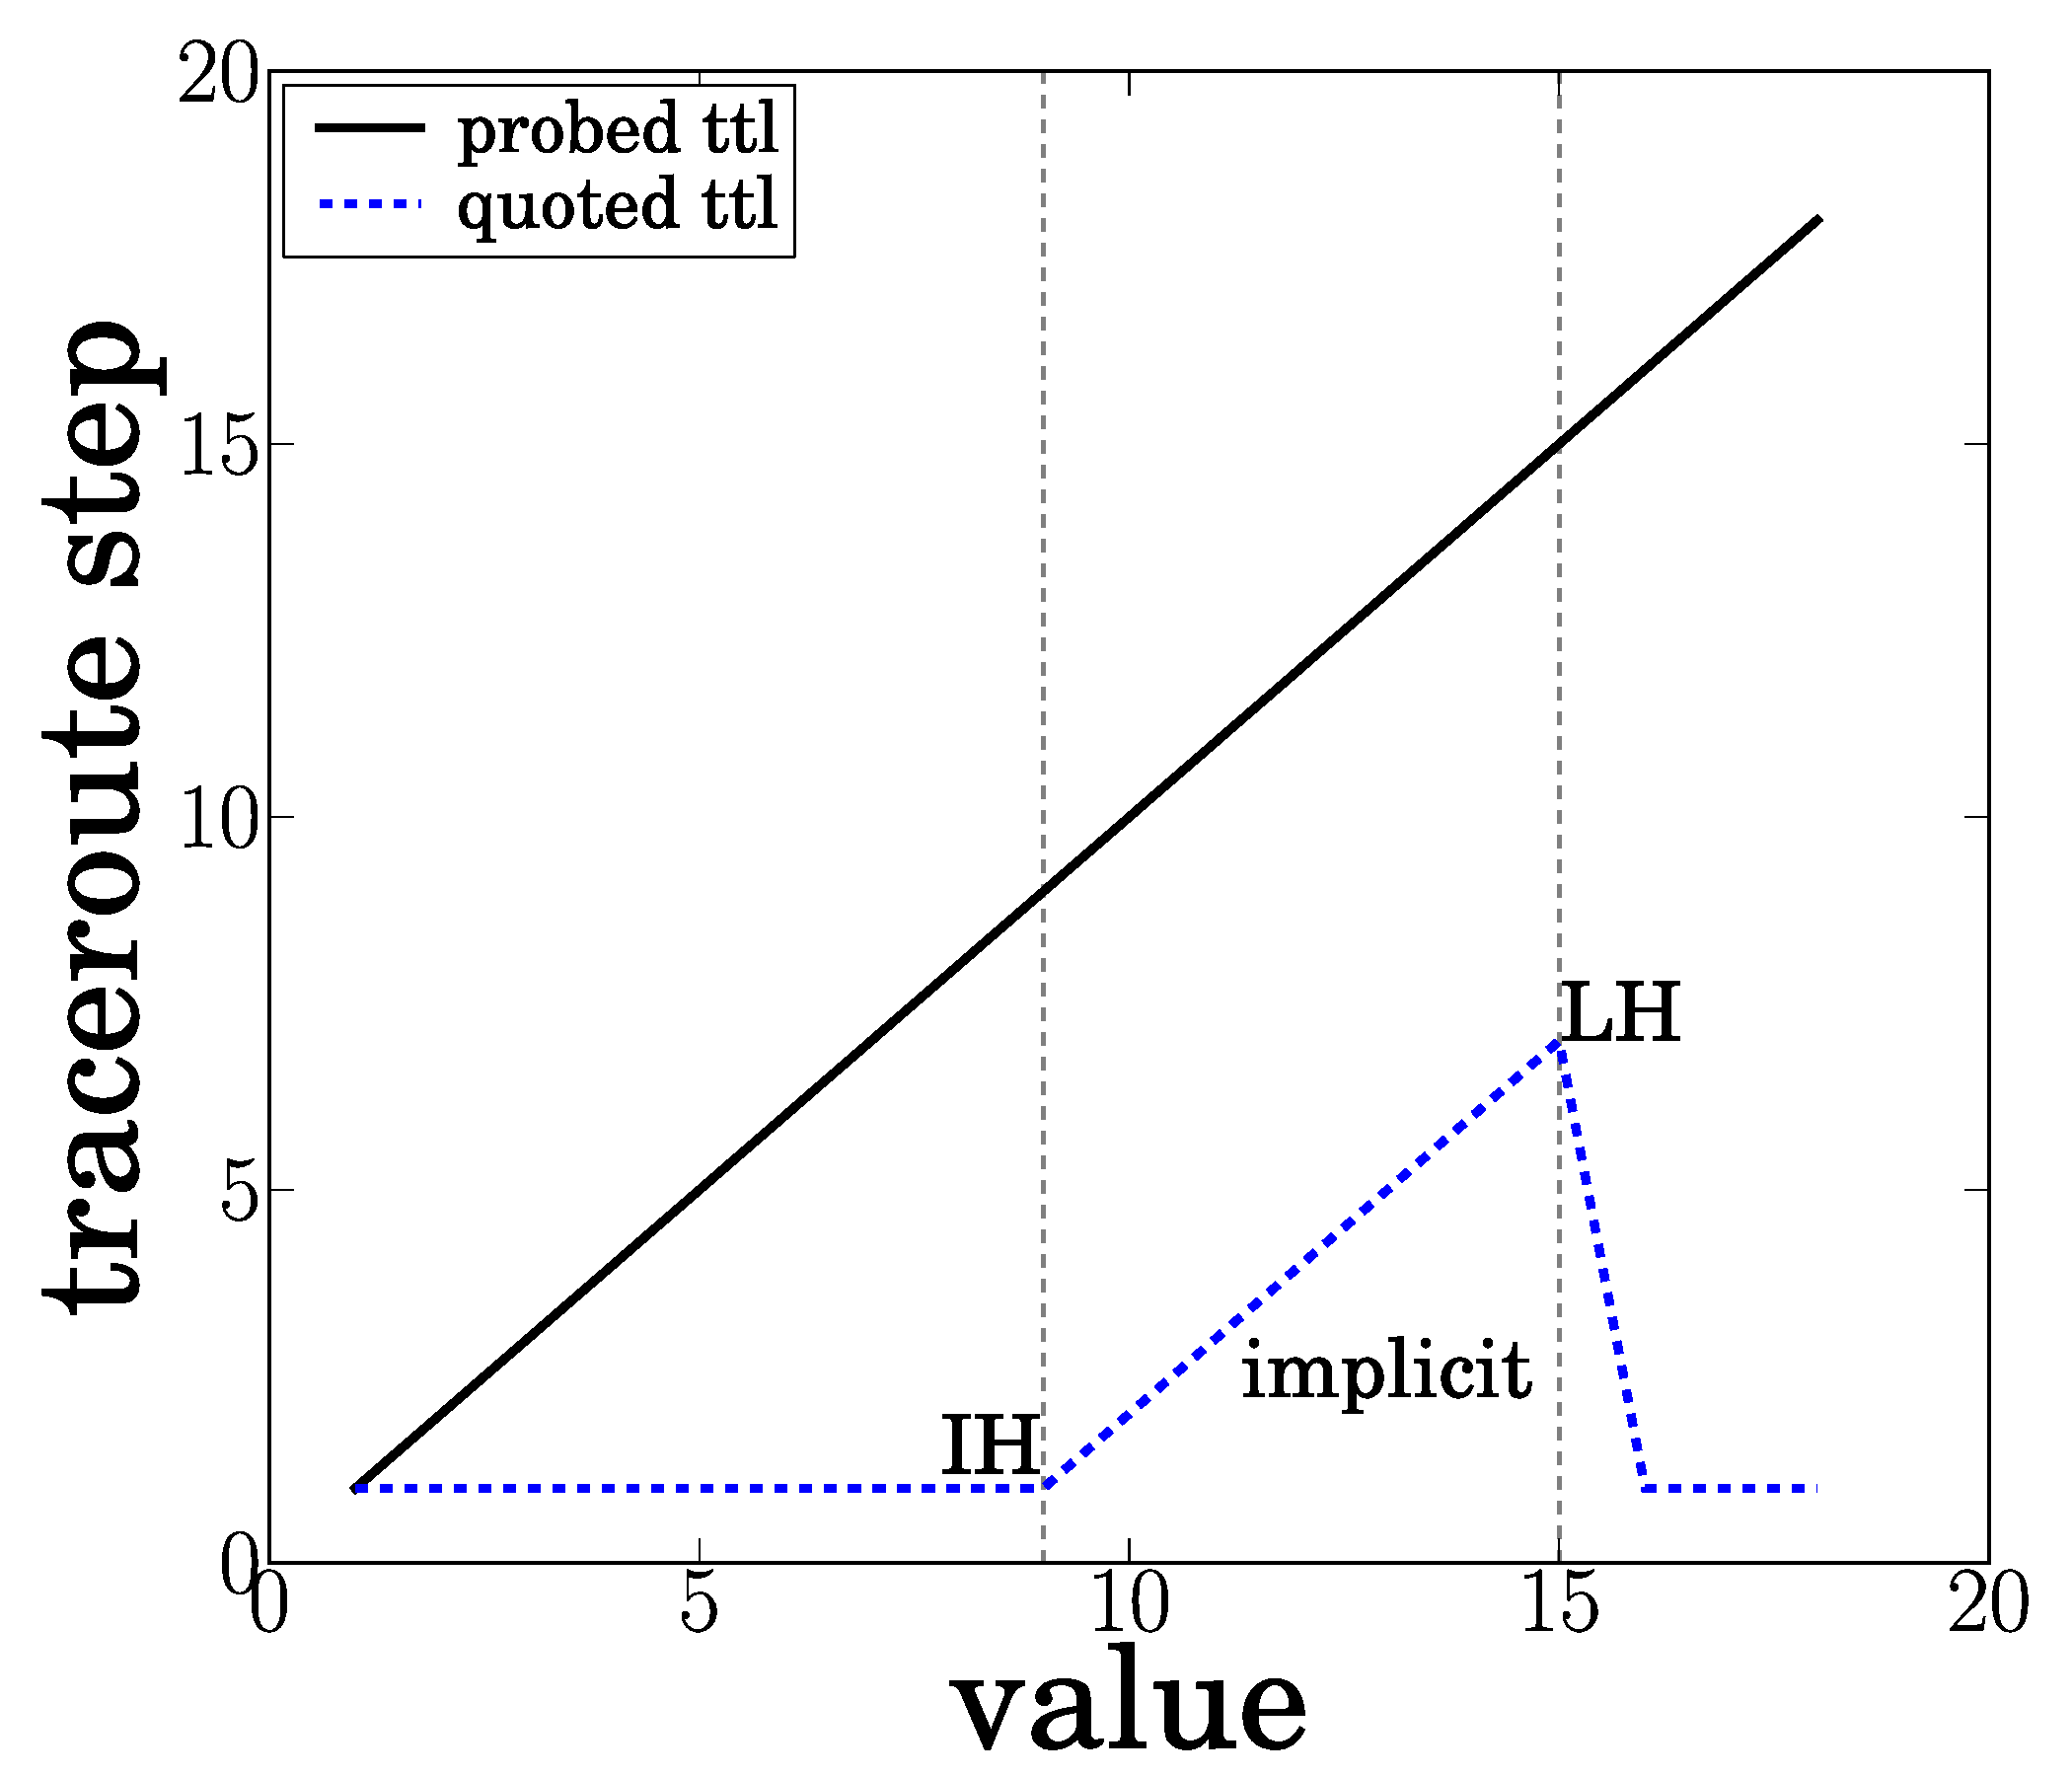
\includegraphics[width=4cm]{QuotedTTL}
%  \end{center}
%  \caption{}
%  \label{validation.qTTLFig}
%\end{figure}




\begin{figure}[!t]
  \begin{center}
    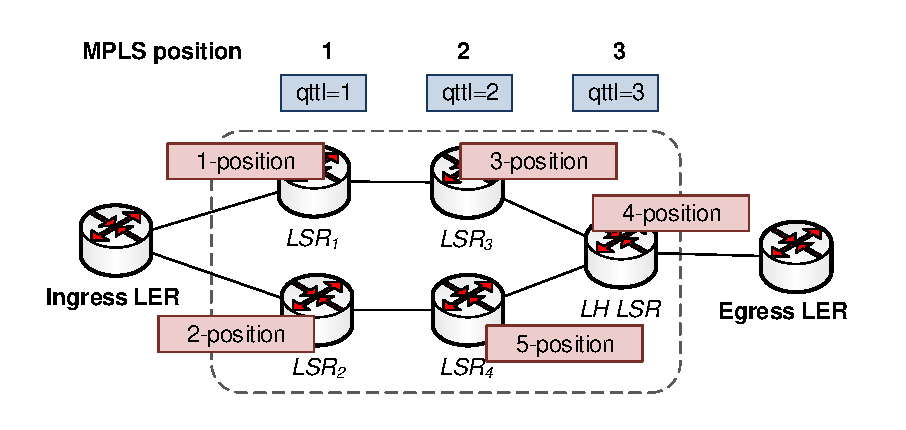
\includegraphics[width=8cm]{mpls_position}
  \end{center}
  \caption{Example of biased $n$-position. Our assumption consider that $n$-position match with the real MPLS position. However, we need first to verify this hypotesis in order to be sure that the behaviour shown on this figure is not a common issue. The figure shows a scenery where due to load balancing issues on the Ingress LER, the $n$-position could be erroneously inferred: First, the traceroute reveal the $LSR_{1}$ ($1$-position), the next traceroute probe reveals the $LSR_{2}$ ($2$-position) and so on.}
  \label{validation.MPLSpositionFig}
\end{figure}

In this section, we expose our methodology for validating the MPLS
signatures used to reveal implicit MPLS tunnels (see Sec.~\ref{related.revealing}).
Basically, we compare the LSR position within an MPLS tunnel, called the
\dfn{MPLS position} with the different signatures values. Our main goal is to test 
u-turn accurancy. Theorically, given an LSR we could get its MPLS position through 
either its qTTL or its u-turn signature. Then, knowing the qTTL value of the LSR we 
can validate its u-turn signature (if any) or vice versa. However, on LSRs revealed 
only trought u-turn signatures,
qTTL values are not present so we need another way to know the related MPLS position. 
Thereby, we assume that the MPLS position
could be obtained independently of the signatures values. 
Thus, we obtained the MPLS position based on the appearance order that a LSR is 
revealed by traceroute and we called to this value $n$-position, i.e., 
The first LSR revealed by a traceroute probe should be
the first LSR within the LSP ($1$-position) , the LSR revealed by the next 
consecutive traceroute probe should be
the second LSR within the LSP ($2$-position), etc. Initially, we consider 
this just as an hypothesis because we do not know 
exactly the MPLS tunnel behaviour in regards with load balancing or others 
unexpected issues, i.e, unexpected load balancing behaviour could cause 
that the appearance order by an LSR in the traceroute ($n$-position) 
is biased in respect to the real MPLS position (see Fig.~\ref{validation.MPLSpositionFig}).

Implicit tunnels are based either on qTTL or u-turn signatures. Both of them are
directly related with MPLS position.  Indeed, first, the qTTL value refers to
the IP-TTL of the \echorequest packet when it enters the MPLS tunnel. 
Therefore, a qTTL of $n$ in the resulting ICMP \ttlexceeded means that the sent
probe expired $n$ hops later than the Ingress LER of the LSP, i.e., an LSR reply
with qTTL$=n$ means that the LSR appears in the \dfn{$n$-position} in the LSP. 
This is illustrated in Fig.~\ref{validation.qTTLFig}.  From the Ingress LER, the
qTTL starts to grow linearly with the LSP length.  We therefore expect observing
a qTTL=$1$ on the first LSR in the LSP, a qTTL$=2$ on the second LSR in the LSP,
etc.  Second, a u-turn value is related to the tunnel length, $L$, and the
$n$-position of the LSR within the tunnel (see Sec.~\ref{related.revealing}) as is shown on Fig.~\ref{validation.uturn1Fig}.

\subsection{qTTL Signature}\label{validation.qttl}
%%%%%%%%%%%%%%%%%%%%%%%%%%%
\begin{figure}[!t]
  \begin{center}
    \subfigure[Tunnel length distribution]{\label{hist_length}
      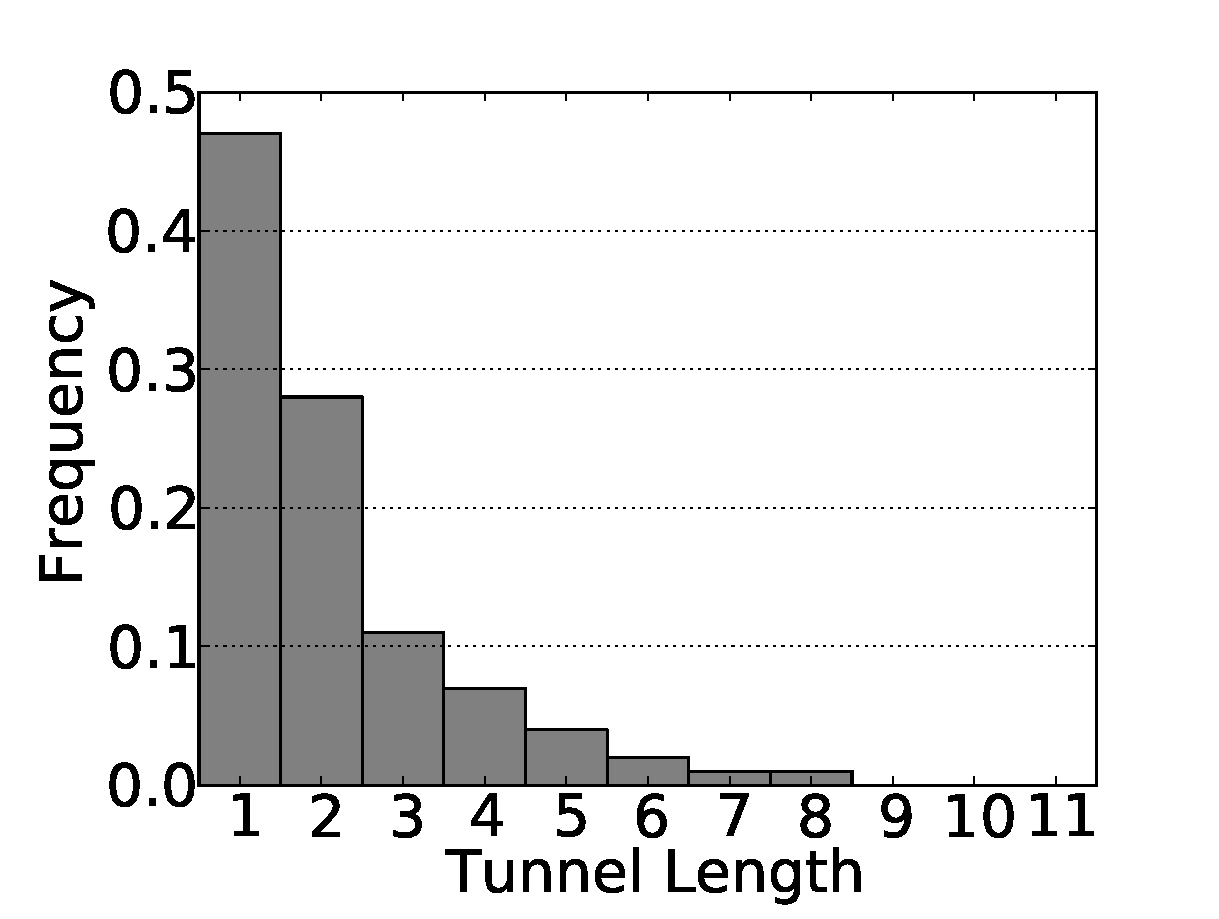
\includegraphics[width=4.3cm]{hist_length}}
\hspace{-0.3cm}      
    \subfigure[qTTL and $n$-position comparison]{\label{n_vs_qttl}
      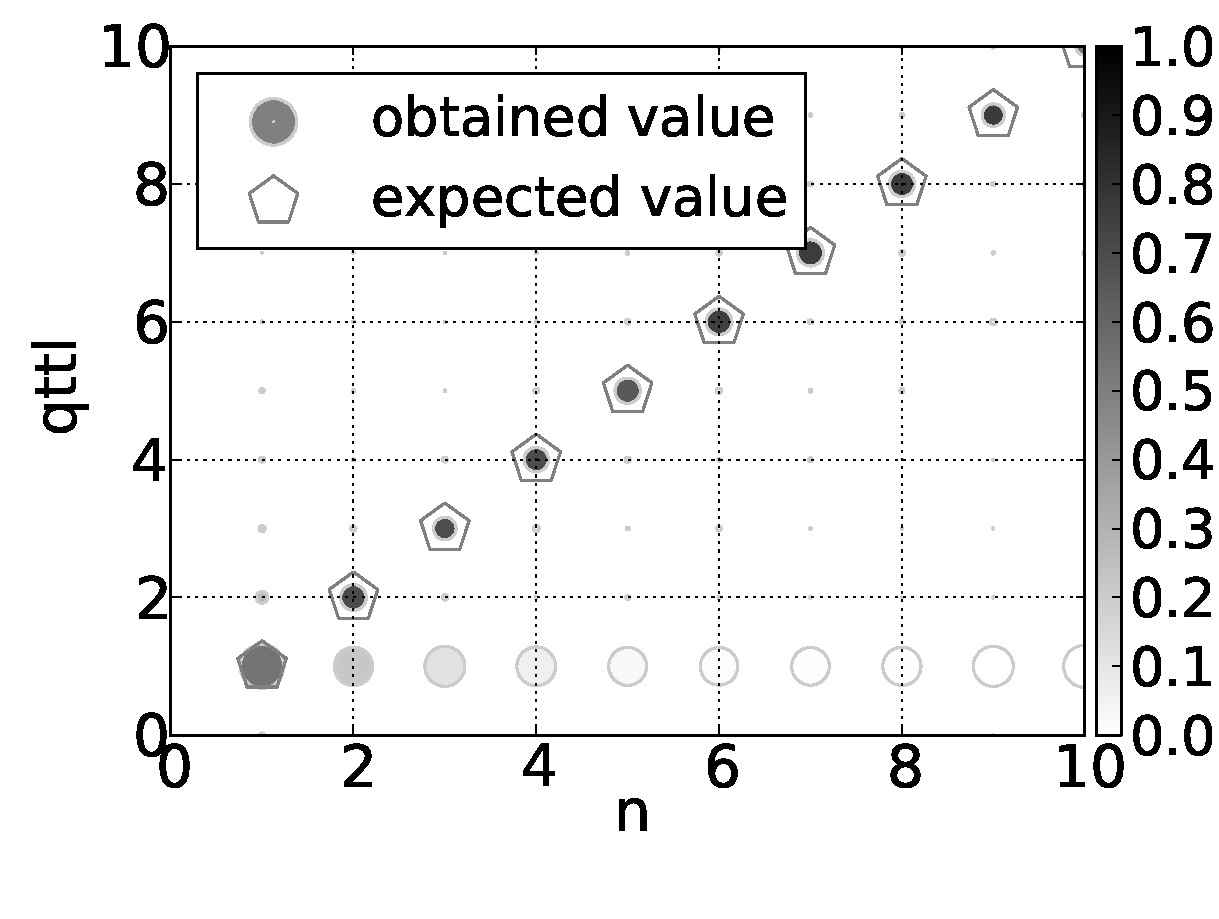
\includegraphics[width=4.3cm]{n_vs_qttl}}  
  \end{center}
  \caption{Comparison between obtained and expected values for qTTL and u-turn.}
  \label{validation.qttl.fig}
\end{figure}

Our signature validation relies on the hypothesis that the real MPLS position matches
with our $n$-position, i.e., the $n$-position of the LSR within the LSP corresponds 
to the qTTL value generated by that LSR. 
Said differently qTTL = $n$.

In order to validate this assumption, we use the dataset described in
Sec.~\ref{dataset} and compare the qTTL with $n$-position for explicit and implicit tunnels \ed{We compare also with explicit tunnels, the exact filter is: RFC4950 IS ON OR QTLL>1. Mainly, we do this in order to add information realted with the amount of those explicit tunnels with have QTTL and those who dont (QTTL=1)}. The results are shown in Fig.~\ref{validation.qttl.fig}.  In
particular, Fig.~\ref{hist_length} provides the MPLS tunnel length distribution
computed as the number of LSRs in the tunnel.  We observe, confirming so
previous studies~\cite{SOM11,Vanaubel15,Donnet12}, that most of tunnels are
rather short (length $< 3$ in more than 80\% of the cases). 

Fig.~\ref{hist_length} also provides, by extension, possible values for qTTL
(X-axis).  This suggests thus that qTTL values should oscillates between 1 and
8, with a strong predominance for short values (i.e., between 1 and 3). 

Fig.~\ref{n_vs_qttl} represents a scatter plot showing the relations between the
qTTL (Y-axis) and the $n$-position (X-axis).  The circle size in the scatter
plot is related with the occurrence frequency of Y-axis values regarding each
$n$-position.  The transparency of the circle is related with occurence
frequency of the $n$-position regarding each Y-axis value.  For instance, on
Fig.~\ref{n_vs_qttl} for values where $n>1$, the biggest circles are mainly
located on qTTL$=1$ and qTTL=$n$.  So, this suggests that, for a given
$n$-position, the qTTL value usually takes either the value $1$ or $n$.

However, we notice, on Fig.~\ref{n_vs_qttl} that the qTTL signature highly
matches with $n$.   The bias $\textit{qTTL}=n \pm \epsilon$ could occur due to
two causes: one is the limitation in our method to reveal the first LSR in the
LSP when RFC4950 is not implemented (by definition of implicit tunnel); and the
second cause could occur due to load balancers (using Paris traceroute should
avoid load balancing issues, except for ``per packet'' load balancers).
In the later case, the \traceroute probes may follow paths with different
lengths before reaching the MPLS tunnel, yielding that the same qTTL value is
revealed several times in different $n$-positions. Fig.~\ref{n_vs_qttl} also
shows that qTTL frequently takes the value of $1$, even for $n>1$, which means
that the LSR implements the RFC4950 but do not mach with the qTTL signature.

%which is consistant with tunnel length distribution (see Fig.~\ref{hist_length}).  \ed{we founf several explicit tunnels where the LSRs just implement RFC4950 but do not have qTTL (qTLL=1 for all positions), so the tunnel lenght is not directly related with the qTTL value, for example: a tunnel with L=3 where LSR1(qTTL=1), LSR2(qTTL=1), LSR3(qTTL=1)}. 

We also find that around $2\%$ of LSRs do not react to qTTL signature, even
if their neighbours does, i.e., some LSRs interfaces located at
$i_{n \pm 1}$ tunnel positions react properly to qTTL signatures but the LSR
interface located at $i_n$ position does not.


Nevertheless, the $n$-position is highly reliable. Indeed, we find that in
$58\%$ of the cases the $n$-position matches with the qTTL value while in
$36,3\%$ of cases the qTTL signature is not present on explicit tunnels and takes the value of $1$,
and just $6,7\%$ of the cases presented have some bias around the expected value
$n$. Those results support our hypothesis: the  MPLS tunnel position highly
matches with the $n$-position. Thereby,  we use $n$-position as a reference
value to validate the u-turn signatures.

\subsection{u-turn Signature}\label{validation.uturn}
%%%%%%%%%%%%%%%%%%%%%%%%%%%%%%

%\begin{figure}[!t]
%  \begin{center}
%    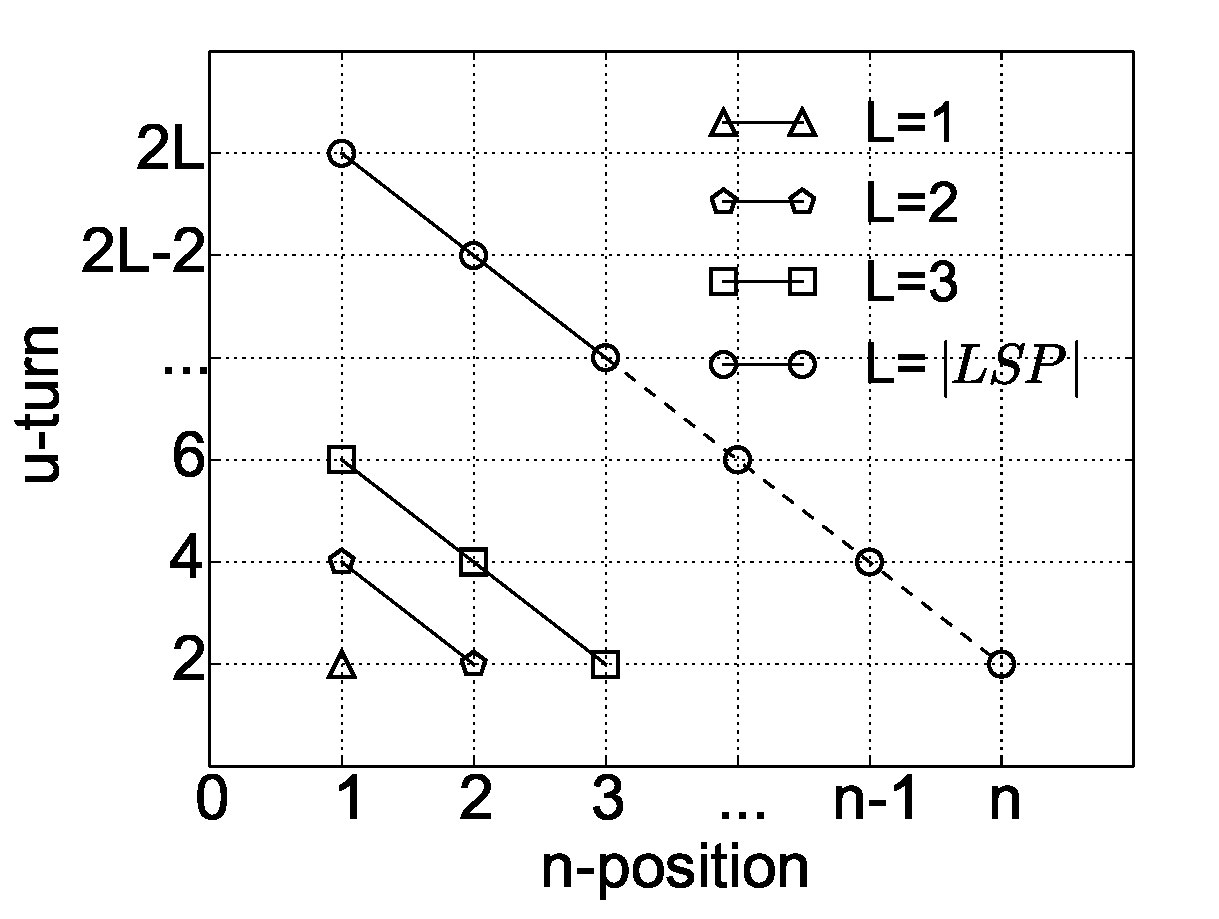
\includegraphics[width=4.3cm]{uturn1}
%  \end{center}
%  \caption{Example of u-turn signature for an implicit MPLS tunnel.}
%  \label{validation.uturn1Fig}
%\end{figure}

\begin{figure}[!t]
  \begin{center}    
    \subfigure[u-turn on LSRs revealed through RFC4950 and qTTL]{\label{fig_uturn_a}
      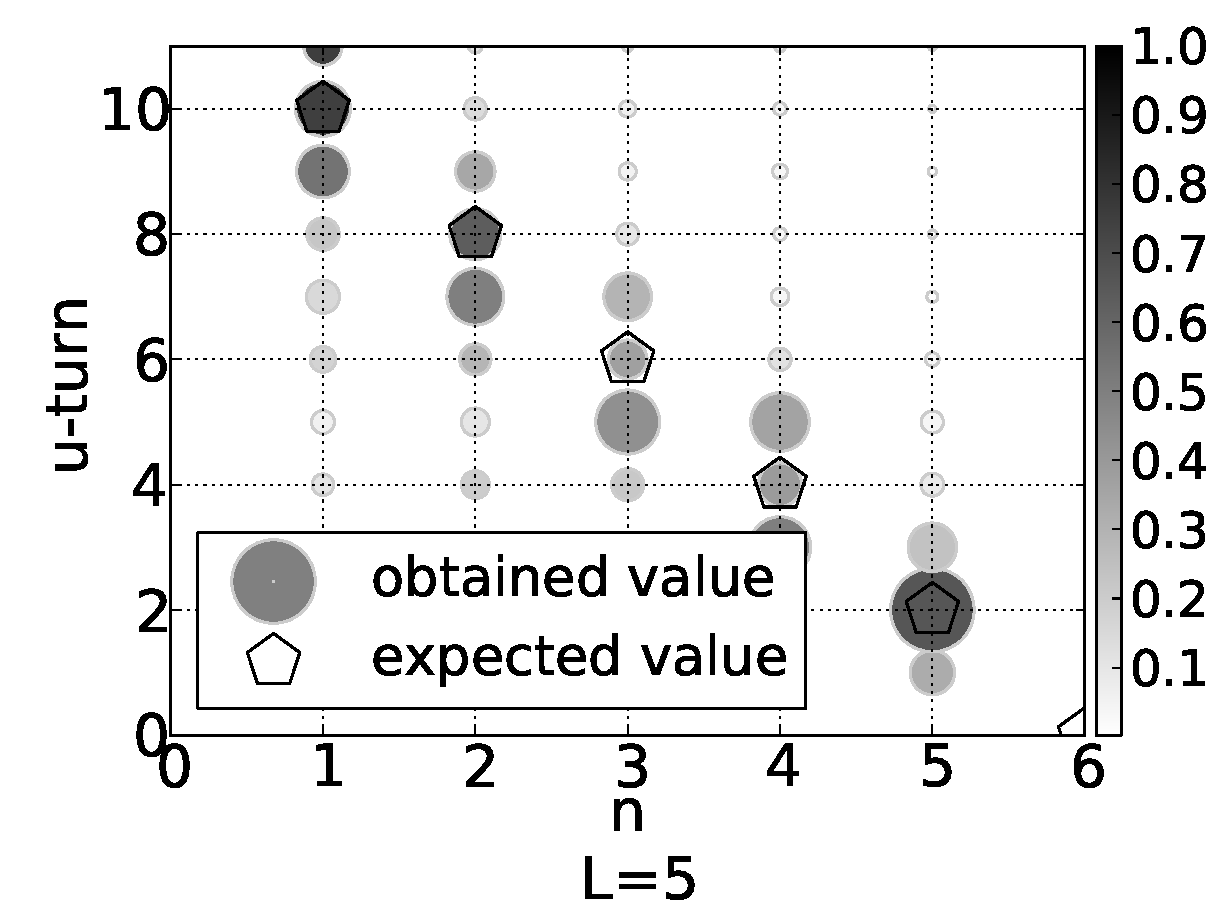
\includegraphics[width=4.3cm]{n_vs_uturn_L5_exp}}
\hspace{-0.3cm}      
    \subfigure[u-turn on LSRs where no other signature was found]{\label{fig_uturn_b}
      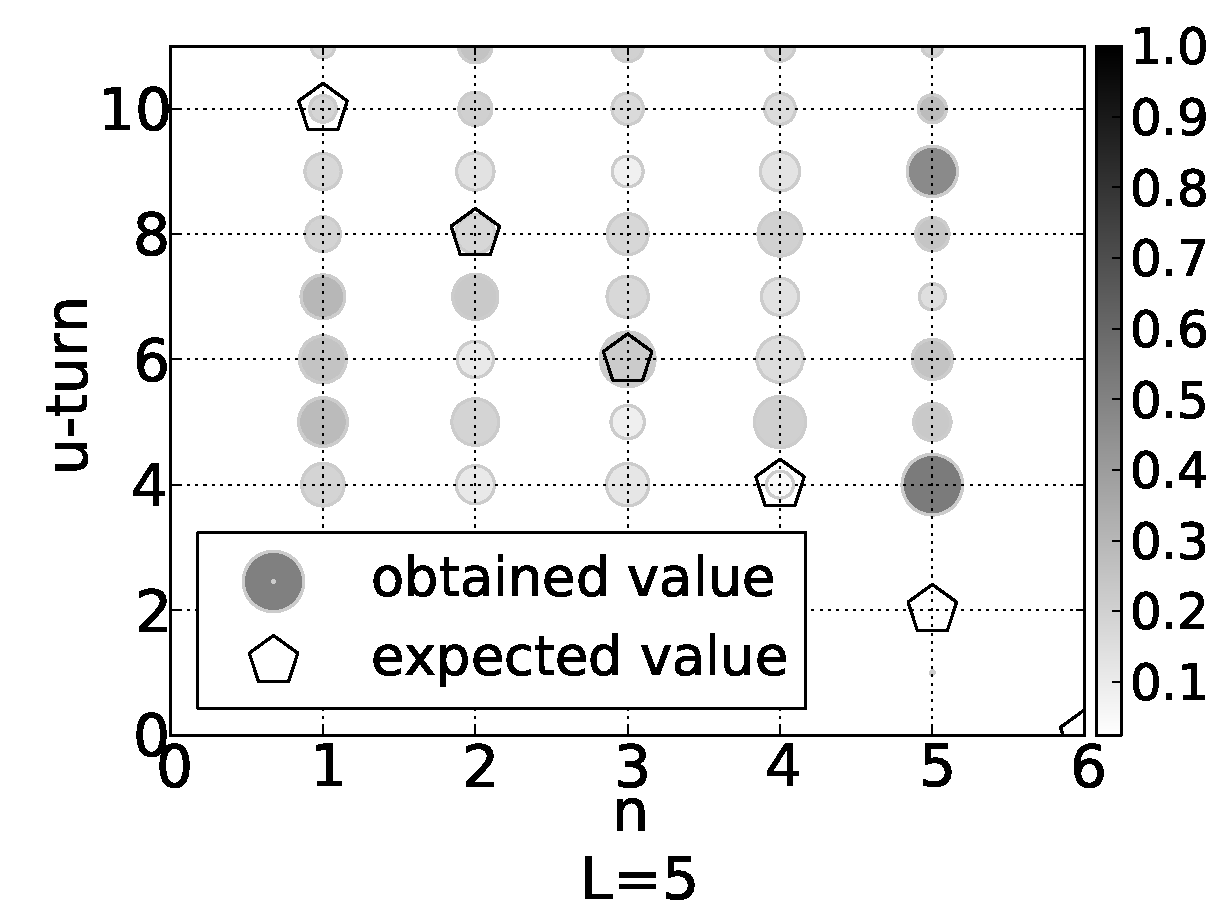
\includegraphics[width=4.3cm]{n_vs_uturn_L5}}
  \end{center}
  \caption{Comparison between obtained and expected values for u-turn
  signature.}
  \label{validation.uturn.fig}
\end{figure}

As explained in Sec.~\ref{related.revealing},  the expected u-turn value is in
the form $[2L, 2L-2, 2L-4,..., 2]$ where $L$ is the tunnel length and the array
position corresponds to the LSR position within the LSP, i.e., $n$ ((see Fig.~\ref{validation.uturn1Fig})).  The
relationship between $L$, $n$, and the expected value can thus be written as
follows:
\begin{equation}
u-turn = 2 \times (L - (n-1)) .
\label{eqn.uturn}
\end{equation}

\ed{This relationship might not look like obvious at first glance.  If we have
room, we should add a figure to illlustrate (as done for qTTL above).}

\ed{An illustration was added. Later, when the corrections are finished, we need to discuss about the space and pages}

Because u-turn is commonly present in almost all LSRs, first, we compare $n$
with u-turn on LSRs revealed either explicitly or qTTL-based using the dataset
presented in Sec.~\ref{dataset}. Later, we also study  $n$ value on LSRs where u-turn
was the only detected signature. We use the filter $\textit{u-turn}>3$ (i.e.,
avoiding so short tunnels where bias are more likely to appear) to avoid false
positives.

The results for a given tunnel length $L=5$ are shown on
Fig.~\ref{validation.uturn.fig}, a scatter plot that must be read the same way
as Fig.~\ref{n_vs_qttl}.  In a few words, Fig.~\ref{validation.uturn.fig}
suggests that u-turn is usually overestimated.  \ed{I stopped here (next
should be rephrased) as I was running out of time.}


Similar results where observed for other lengths ($L$). Basically, we noticed
that  obtained u-turn values are close to expected ones when
the LSRs was either explicitly revealed or qTTL is present
(Fig.~\ref{fig_uturn_a}). However, on the set of LSRs revealed only by u-turn
signatures (Fig.~\ref{fig_uturn_b}) the obtained and expected u-turn values  
commonly does not match. If we accept a bias of $ \pm 2$ around the expected
u-turn value, we noticed that on LSRs explicitly revealed and qTTL based, 
the $60\%$ of obtained u-turn signatures match with the
expected values. However, on LSRs revealed only trough
u-turn signature (therefore where it is really useful), the obtained u-turn
cases just match in less than $25\%$ of cases with the expected values ($2(L-(n-1))$).
Therefore, LSRs revealed only through u-turn is highly inaccurate; mainly,
because MPLS tunnels are not the only responsible of u-turn signature aparition but
it is also related with load balancing issues in the return path. Basically, 
the two kinds of messages related with u-turn signatures (ICMP \echoreply  and ICMP
\ttlexceeded) belong to diferents balancing \textit{flows} and thereby follow different return paths. 

%is common for paths between the same pairs
%source-destination \cite{BRICE07}. This issue is called \dfn{per-flow} load
%balancing. Basically, packets that belongs to the same \dfn{flow} are treated
%similarly \cite{BRICE06}. A flow is identified by the first 32 bits of the IP
%\textit{payload}, e.g., TCP header. In the case of ICMP messages, this fields
%refers to \texttt{Type}, \texttt{Code}, and \texttt{Checksum}.
%By definition, u-turn signature is based on two kinds of ICMP messages:
%ICMP \echoreply \texttt{Code 11} and ICMP \ttlexceeded \texttt{Code 0}.
%Due to different codes for each ICMP message, there is no way to assure that
%they belong to the same flow identifier and thereby to be sure that u-turn value
%is caused just by MPLS tunnels.  \ed{The full explanation of ``per flow'' is not
%required (we can assume people are familiar with this).  But we have to clearly
%state that this is during the ``return'' path (i.e., from the LSR generating the
%\ttlexceeded towards the VP) that those per-flow LB can mainly occur.
%Otherwise, I miss something here.}

\section{LSRs and \textit{MPLS clusters}}\label{cluster}
% %%%%%%%%%%%%%%%%%%%%%%%%%%%%%%%%%%%%%%
To the best of our acknowledge, MPLS interconnection architecture on Internet
topology has not yet been studied. Our study aims at better
understanding the impact of MPLS deployments over Internet, specifically over
router level topology. First, we study how LSRs and \dfn{MPLS clusters} 
interacts  with the entire Internet Topology . Secondly, we
study the MPLS clusters behaivor given a specific AS.

\subsection{Definitions and Background}\label{cluster.methodo}
% %%%%%%%%%%%%%%%%%%%%%%%%%%%%%%%%%%%%%%
\begin{figure*}[!htb]
  \begin{center}
    \subfigure[Degree Distribution Probability]{\label{fig_degree_distribution}
      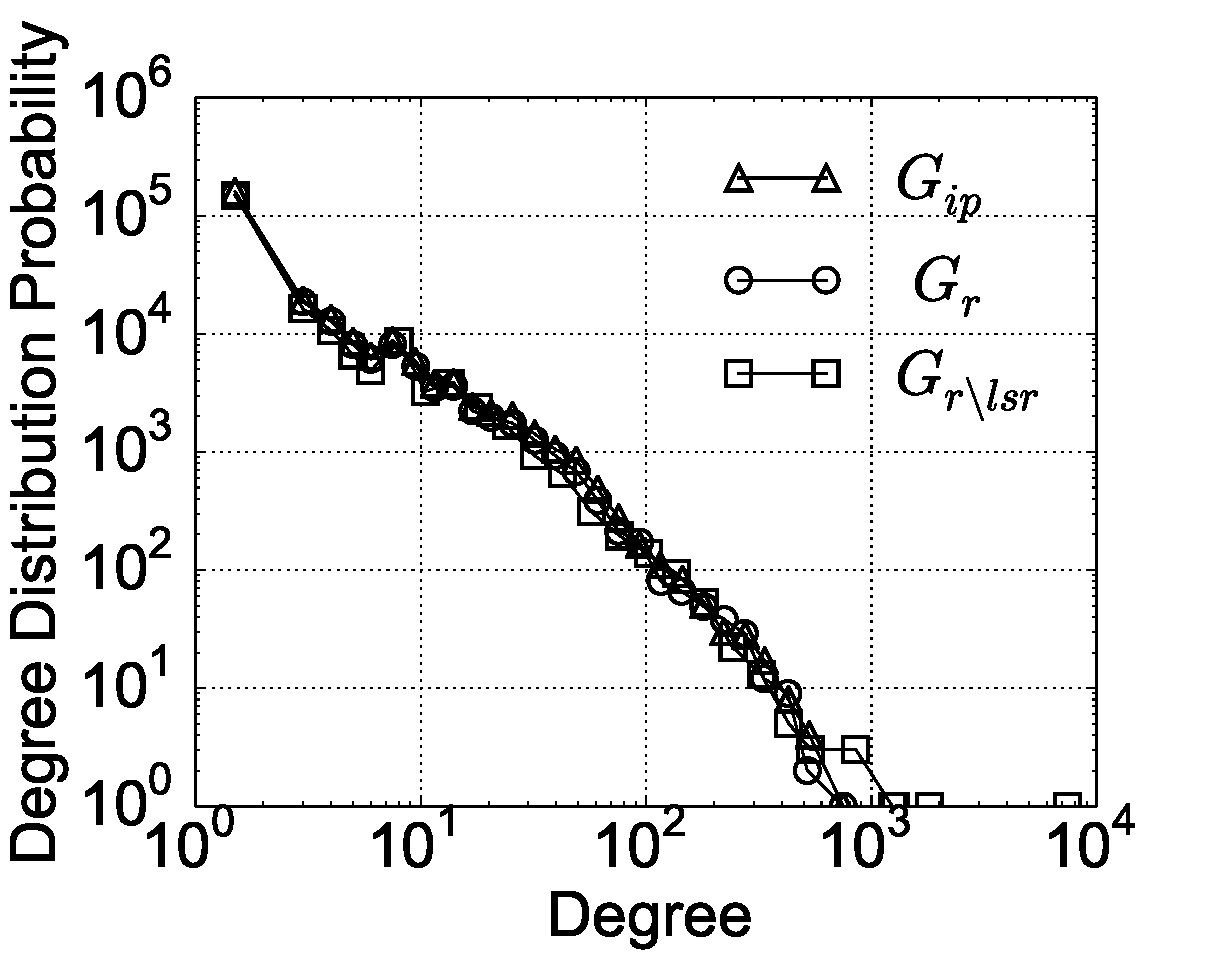
\includegraphics[width=5.5cm]{DegreeDistribution}}\hfil
    \subfigure[Clustering Coefficient]{\label{fig_clustering}
      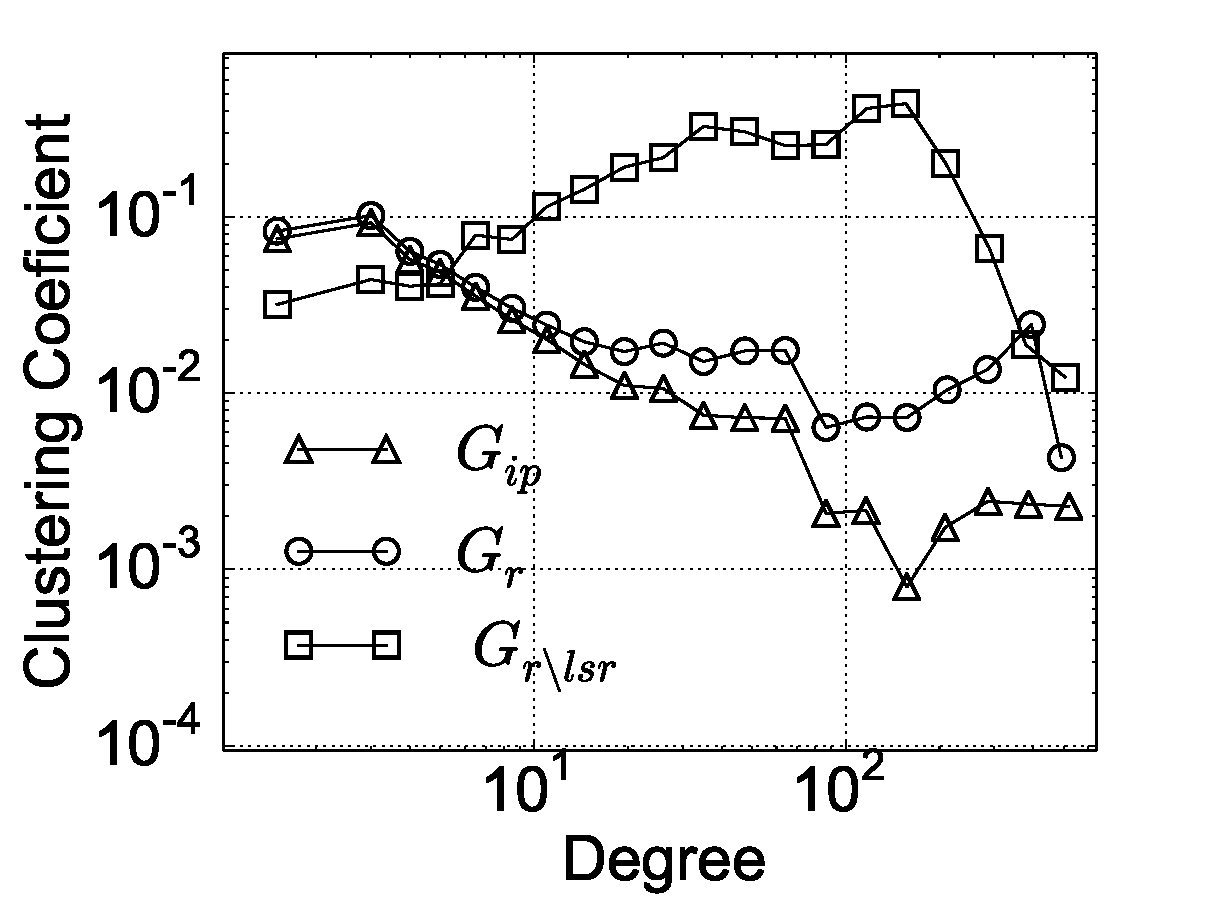
\includegraphics[width=5.5cm]{ClusteringCoeficient}}\hfil
    \subfigure[Neighbor Degree Distribution]{\label{fig_neighbor}
      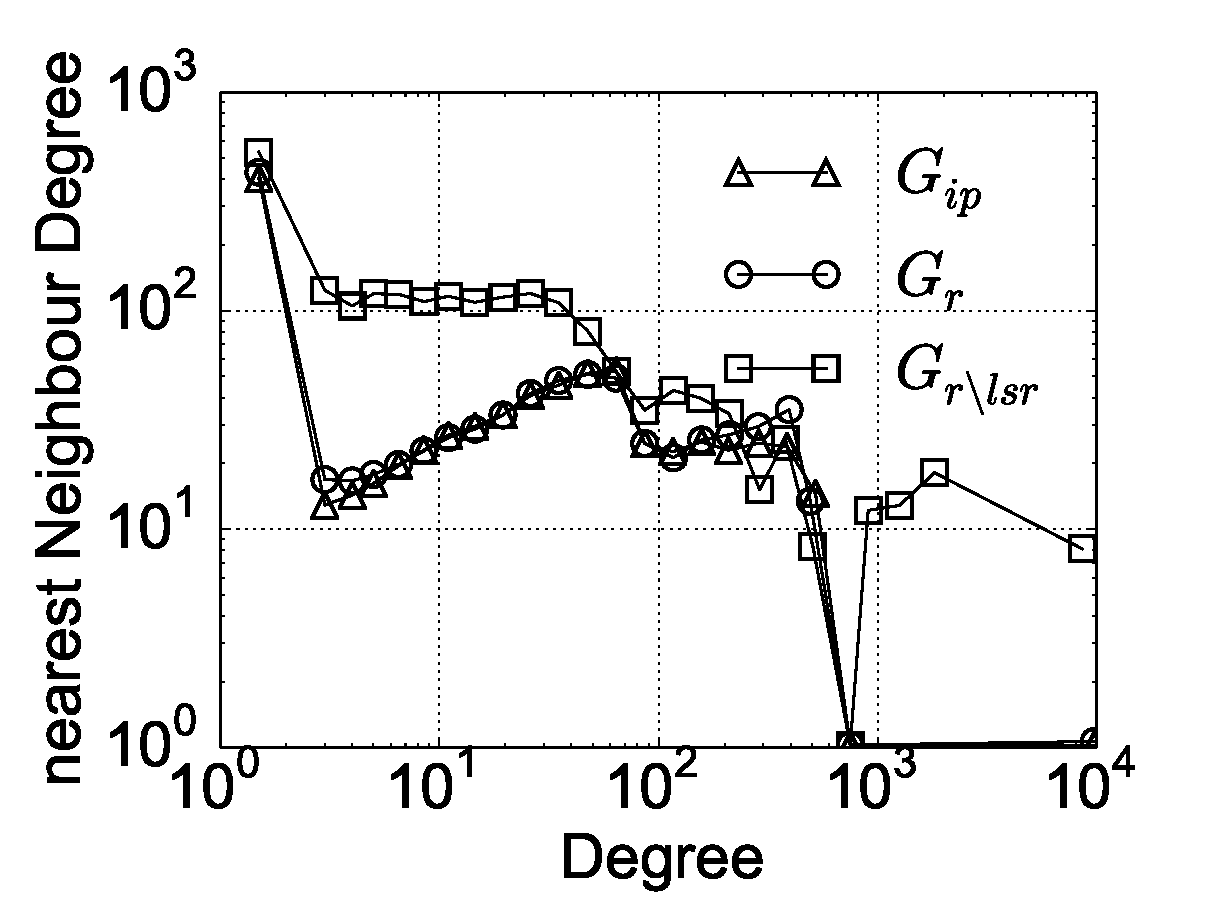
\includegraphics[width=5.5cm]{NearestNeighbor}}
  \end{center}
\caption{Metrics for IP, router and MPLS cluster interconnection
topologies.} 
\label{fig_metrics}
\end{figure*}

\begin{table}[!t]
  \begin{center}
    \begin{tabular}{l|ll}
    \textbf{Graph} & \textbf{Notation} & \textbf{Definition}\\
    \hline
    IP                 & $G_{ip}$ & $(V_{ip}, E_{ip})$\\
    Router             & $G_r$ & $(V_r, E_r)$\\    
    MPLS               & $G_r^{mpls}$ & $(V_r^{mpls}, E_r^{mpls})$\\
    ASes induced graph & $G_r(as)$ & $(V_r(as), E_r(as))$\\    
    MPLS cluster       & $C_i^{mpls}$ & /\\
    MPLS cluster interconnection graph & $G_{r \backslash lsr}$ & $(V_{r
    \backslash lsr}, E_{r \backslash lsr}^{mpls})$
    \end{tabular}
  \end{center}
  \caption{Summary of graph notations used in Sec.~\ref{cluster}.}
  \label{cluster.table_notations}
\end{table}




We defined several graphs at different abstraction levels as follows (they are
summarized in Table~\ref{cluster.table_notations}): The \dfn{IP level graph} $G_{ip}$, builded
by the IP addresses and links found trough
\traceroute. Second, the \dfn{router level graph} $G_{r}$ (alias resolution having been done
through MIDAR~\cite{Keys13}). Third, the \dfn{MPLS router level
graph} $G^{mpls}_{r}$, formed by MPLS links and routers in which at least one IP interface belongs
to an LSP.


%We defined several graphs at different abstraction levels as follows (they are
%summarized in Table~\ref{cluster.table_notations}): The \dfn{IP level graph} is
%defined as $G_{ip}=(V_{ip}, E_{ip})$, where $V_{ip}$ is the IP addresses
%discovered in our exploration and $E_{ip}$ the set of the links found trough
%\traceroute. Second, the \dfn{router level graph} is defined as $G_{r}=(V_{r},
%E_{r})$, where $V_{r}$ is the set of routers (alias resolution having been done
%through MIDAR~\cite{Keys13}), and $E_{r}$ is the set of all the links found
%between any pair of routers $v \in V_{r}$. Third, the \dfn{MPLS router level
%graph} refers to $G^{mpls}_{r}=(V^{mpls}_{r}, E^{mpls}_{r})$ where
%$V^{mpls}_{r}$ is the set of routers in which at least one IP interface belongs
%to an LSP, and  $E^{mpls}_{r}$ is the set of all \textit{mpls links}.
%$(v^{mpls}_{r}(i), v^{mpls}_{r}(j))$ such as
%$\{{v^{mpls}_{r}(i)},{v^{mpls}_{r}(j)} \}\in V^{mpls}_{r}$.

The \dfn{ASes induced graph} $G_{r}(as)$ is a induced subgraph of $G_{r}$ where 
each vertex  has an interface belonging to the same Autonomous System, $as$. 
In particular, the induced graph of $G_r^{mpls}$ is
$G^{mpls}_{r}(as)$.  This definition allows
us to define an \dfn{MPLS cluster}, $C^{mpls}_{i}$, as a connected component $i$
of $G^{mpls}_{r}(as)$. A given AS may have several MPLS clusters.

%The \dfn{ASes induced graph} is defined as $G_{r}(as)=(V_{r}(as), E_{r}(as))$.
%Each vertex in $G_{r}(as)$ has an interface belonging to the same Autonomous
%System, $as$.  In particular, the induced graph of $G_r^{mpls}$ is
%$G^{mpls}_{r}(as)=(V^{mpls}_{r}(as), E^{mpls}_{r}(as))$.  This definition allows
%us to define an \dfn{MPLS cluster}, $C^{mpls}_{i}$, as a connected component $i$
%of $G^{mpls}_{r}(as)$. A given AS may have several MPLS clusters.

Finally, the \dfn{MPLS cluster interconnection graph} is an hybrid router level
graph,  $G_{r\backslash lsr}$,
where all the MPLS clusters $C^{mpls}_{i}$ are gathered together in a single
node, while non-MPLS capable routers remain unchanged.
Broadly speaking, an MPLS cluster interconnection graph refers to a router level
graph where all MPLS clusters are treated as a single node. Additionally,
we call $G_{r\backslash lsr}(as)$ to the induced
subgraphs of $G_{r\backslash lsr}$ by routers having at least one interface in
the Autonomous System $as$.


%Finally, the \dfn{MPLS cluster interconnection graph} is an hybrid router level
%graph,  $G_{r\backslash lsr}=(V_{r\backslash lsr},E^{mpls}_{r\backslash lsr})$,
%where all the MPLS clusters $C^{mpls}_{i}$ are gathered together in a single
%node $v\in V_{r\setminus ls}$, while non-MPLS capable routers remain unchanged.
%Broadly speaking, an MPLS cluster interconnection graph refers to a router level
%graph where all MPLS clusters are treated as a single node. In this way, we can
%study how IP interfaces and non MPLS capable routers interact with MPLS
%clusters. Additionally, we call $G_{r\backslash lsr}(as)$ to the induced
%subgraphs of $G_{r\backslash lsr}$ by routers having at least one interface in
%the Autonomous System $as$.

% \textbf{IP level Graph:} $G_{ip}=(V_{ip}, E_{ip})$, where $V_{ip}$ is the IP
% address discovered in our exploration and $E_{ip}$ is the set of the links found
% trough traceroute. Note that \traceroute just records incident IP addresses in
% a path.

As the analysis is mainly based on $k$-core decomposition, we present the
following definitions:
\begin{itemize}
  \item\dfn{\textit{k}-core:} Given a graph $G=(V,E)$, then the
  subgraph $H=(C,E|C)$ induced by the set $ C\subseteq V$ is a \textit{k}-core
  of order $k$ $iff$ $\forall v \in C: degree_{H}(v)\geq k$ and $H$ is the
  maximum subgraph with this property.
%A \textit{k}-core of $G$ can therefore be obtained by recursively removing all
% the vertices of degree less than $k$, until all vertices in the remaining
% graph have at least degree $k$.    
  \item\dfn{Shell index}. A vertex $i$ has a shell index $c$ if it
  belongs to the $c$-core but not to $(c+1)$-core. We denote by $C_i$ the shell
  index of vertex $i$. A shell $C_c$ consists of all the vertices whose shell
  index is $c$. The maximum value $c$ such that $C_c$ is not empty is denoted by
  $C_{\max}$.  Therefore, the $k$-core is thus the union of all shells $C_c$ with
  $c \geq k$.
\end{itemize}

To retrieve the $k$-core decomposition of a graph $G$, we use
\lanet\cite{Alvarez06k}.  This tool returns a two dimensional plot,
where the position of each vertex depends on its shell index and its neighbors'
index. A color code allows for the identification of shell indices. 
Finally, the size of each node is proportional to the original degree of that vertex; 
\lanet uses a logarithmic scale for the size of the drawn bullets. A central 
role in the visualization method is played by multi-components
representation of $k$-cores.  \ed{It is unclear to me what's a multi-component
representation.  The next sentences in this paragraph are also unclear} In the
most general situation, the recursive removal of vertices having degree less	
than a given $k$ can break the original network into various connected
components, each of which might even be once again broken by the subsequent
decomposition.

In this paper, we use $k$-core decomposition focused on properties around mpls
clusters interconnection. This provides us an idea about the
structural arrangement and topological properties caused by MPLS usage.
Additionally, the visualization helps us to find properties and fingerprints
tightly related with MPLS presence.

\subsection{MPLS on Internet Topology}\label{cluster.topo}
% %%%%%%%%%%%%%%%%%%%%%%%%%%%%%%%%%%%%%%
\begin{figure}[!t]
  \begin{center}
    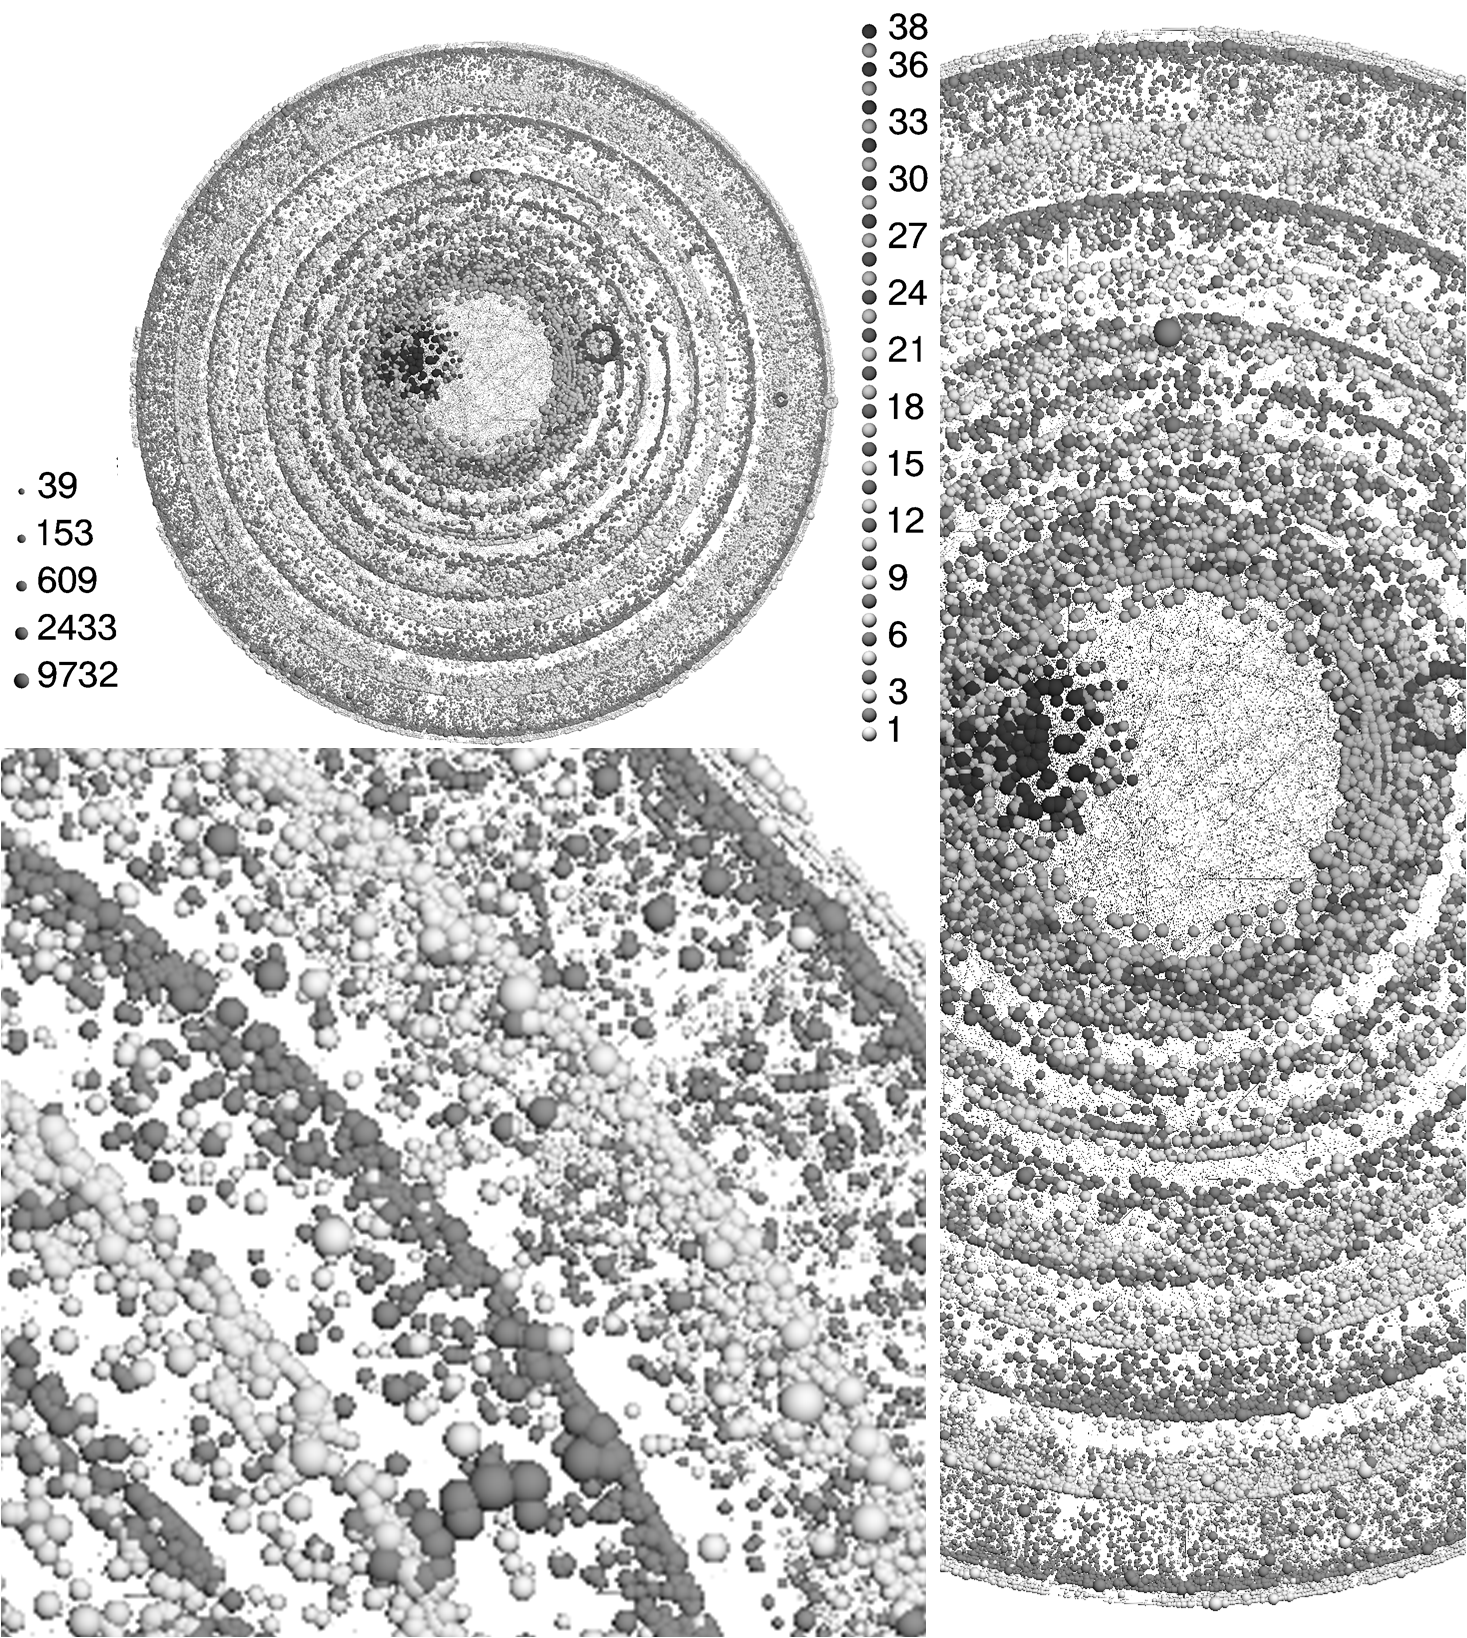
\includegraphics[width=3in]{Routers}
  \end{center}
  \caption{$k$-core visualization of router level topology $G_{r}$.}
  \label{fig_k_core_routers}
\end{figure}

We first analyze the graphs $G_{ip}$ and $G_{r}$ in order to know if there are
some strong differences between their structure and properties. As expected, we
notice that the router level topology has slightly stronger clustering
coefficient than the IP level topology (see Fig.~\ref{fig_clustering}), due to
% the join of IP interfaces into single routers.
alias resolution process.  However, the main structure of both topologies is
similar as displayed on Fig.~\ref{fig_degree_distribution}
and~\ref{fig_neighbor}. Because we do not see any meaningful difference
between these topologies, and the router level topology is closer to a
realistic Internet one, we use the later for the remaining of our analysis.

Fig.~\ref{fig_k_core_routers} shows the $k$-core visualization of $G_{r}$.  The
figure is divided in three parts, the main part being in the upper left while
the two others are a zoom on the main part.  The main part is composed of two
scales, the one on the left is the node degree scale representing the degree in
a logarithmic scale, while the one on the right is a gray scale with each shell
index $c_i$.  Between the two scales, we see the shell index with $C_{\max}$ in
the center, the other shells being located concentrically around it. Note that
$C_{\max}$-core is made of several components with one having the most
significant part, and it is shown at the left of the center (black nodes).  We
also see that all the shells index are highly populated and that the node degree
is not related with the shell index, i.e., there are many routers with high
degree in the outer (lower) shells.  Another typical feature of router level
topology is that the links between routers mainly occurs between routers
belonging to neighbors shells, e.g., the routers on the outer shells are not
usually connected to the routers located on the  $C_{\max}$-core, as it is in
the Autonomous Systems maps~\cite{Alvarez06k}.

\begin{figure*}[!t]
  \begin{center}
    \subfigure[The $k$-core visualization of router level topology $G_{r}$.]{\label{fig_k_core_LSR}
      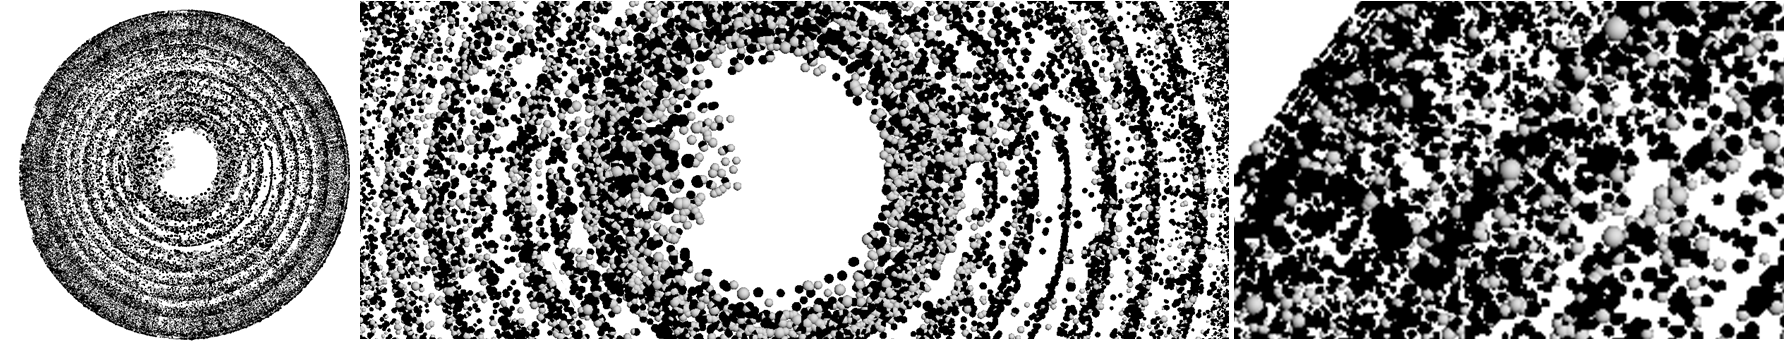
\includegraphics[width=18cm]{LSR}}
\hfil
    \subfigure[The $k$-core visualization of MPLS cluster level topology  $G_{r\backslash lsr}$.]{\label{fig_k_core_MPLS}
      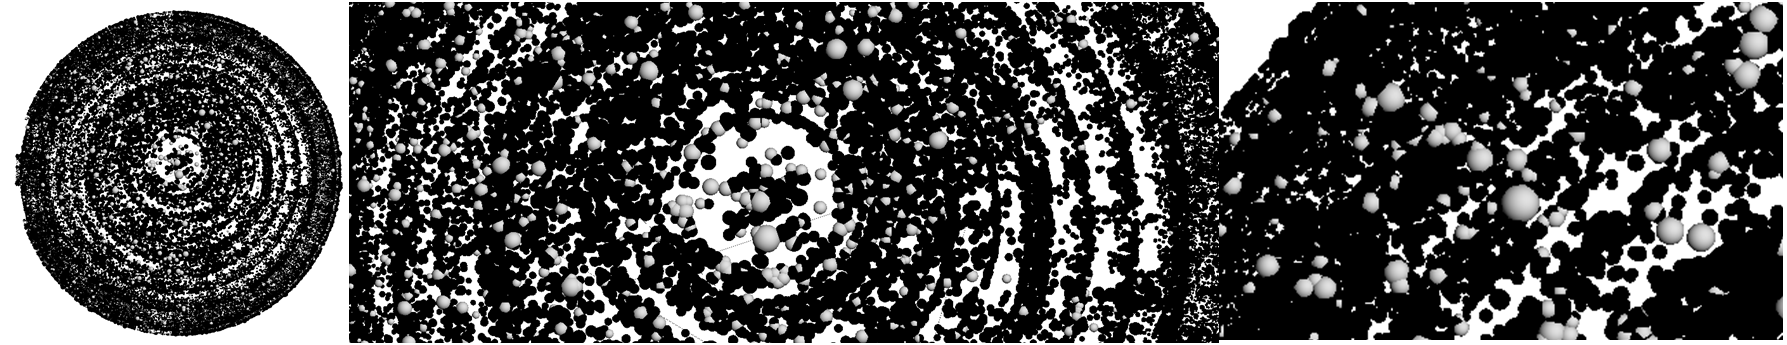
\includegraphics[width=18cm]{MPLS}}
  \end{center}
  \caption{$k$-core visualization of $G_r$ and $G_{r \backslash lsr}$.  On
  Fig.~\ref{fig_k_core_LSR}, black nodes refer to non MPLS capable routers and
  gray nodes refer to LSRs.  On Fig.~\ref{fig_k_core_MPLS}, black nodes refer to
  non MPLS capable routers and gray nodes refer to MPLS clusters.} 
  \label{fig_kcore_overview}
\end{figure*}

In order to locate LSRs-routers with MPLS capabilities into the shells index
over $k$-core decomposition, we paint in black the non-MPLS routers and in gray
the LSRs. The results are showed in Fig.~\ref{fig_k_core_LSR}.  For the sake of
the visualization, we do not include neither the shell index, degree scale, nor
edges between shells. We notice that the LSRs are commonly distributed around
the different shells of Internet but slightly tends to concentrate with more
density nearby the $C_{\max}$-core. Additionally, we apply the same methodology
for the MPLS interconnection cluster level graph $G_{r\backslash lsr}$
(Fig.~\ref{fig_k_core_MPLS}): MPLS clusters (gray nodes) are distinguished from
the non MPLS capable routers (black nodes). In this case,  MPLS clusters  are
also spread out on the Internet.  Indeed, we see some well defined gray nodes on
the periphery of the decomposition. However MPLS clusters show a stronger
tendency to concentrate near the $C_{\max}$-core.

Finally, we evaluate the impact of MPLS clusters on the typical router level
topology, i.e., MPLS cluster interconnection graph $G_{r \backslash lsr }$. We
use metrics such as degree distribution, clustering coefficient, and nearest
neighbor degree, as is shown on Fig.~\ref{fig_metrics}.
We notice that MPLS clusters highly impact over the router level topology. On
one hand, the nearest neighbor degree highly increments for low degrees nodes on
$G_{r \backslash lsr }$, suggesting that routers with low degree are highly
connected to MPLS clusters and thereby to LSRs. On the other hand, the
clustering coefficient of $G_{r \backslash lsr }$ change significantly their
slope in regards with IP and router level topology, indicating that routers with
high degree are connected to \textit{common} MPLS clusters. \ed{does this
suggest that some MPLS clusters are more ``popular'' than others?}

\subsection{\textit{MPLS clusters} on Autonomous Systems}\label{cluster.as}
% %%%%%%%%%%%%%%%%%%%%%%%%%%%%%%%%%%%%%%%%%%%%%%%%%%%%%%%%%
Although, the previous results give us a general overview about MPLS deployment,
we believe that the study of MPLS structure requires to go deeper into the
individual AS topology. Indeed, we found that around $89.9\%$ of \textit{mpls
links} are intra-domain. Thereby, we focus on the top ASes in terms of total
number of discovered links.  On this set of ASes, we discard those having less
than 500 mpls links. Additionally, we identify the amount of discovered MPLS
links by AS, distinguishing the type of MPLS tunnel to their belong i.e., given
a link between two MPLS interfaces $i_{n-1}$  and $i_{n}$ discovered by 
traceroute at $n-1$ and $n$ position, we called:

\begin{itemize}
  \item[i] \textit{explicit mpls link:} links 
  where $i_{n}$ belongs  to an explicit MPLS tunnel.
  \item[ii] \textit{qTTL mpls link:} links 
  where $i_{n}$ belongs  to an implicit MPLS tunnel qTTL based.
  \item[iii] \textit{u-turn mpls link:} links 
  where $i_{n}$ belongs  to an implicit MPLS tunnel u-turn based.
\end{itemize}

The summary of the top ASes is showed in the Fig.~\ref{top_as}.
We noticed that the ratio $r_{mpls}= \vert E^{mpls}_{r} (as) \vert /\vert E_{r}
(as) \vert $  is greater when more  \textit{explicit mpls links} have been
discovered. Interestingly, we also see that the ASes with more links discovered
have the lowest ratio $r_{mpls}$.

For our purposes, we select the most representatives ASes from those in
Fig.~\ref{top_as}. In this way we analyzed the graphs $G_{r}(as)$ and
$G_{r\backslash lsr}(as)$ for AS1299, AS174, AS6762, AS2914, AS7018 and AS1273.
The most remarkable observation (see Fig.~\ref{fig_cluster_mpls}) occurs
regarding the graph $G_{r\backslash lsr}(as)$: $k$-core decomposition highly
differs on those ASes, where prevails explicit tunnels in regard to those with
more \textit{u-turn} tunnels proportionally. We show that \textit{MPLS clusters}
(represented as gray nodes) for  AS1299 (Teliasonera AB), AS174 (Cogent
Communication) and AS6762 (Telecom Italia) are spread out over different shells
index. These $k$-core structures are similar in our top four of ASes where we
additionally noticed  the \textit{u-turn} signature was majority discovered,
i.e., between $30\%$ and  $80\%$ over  the total amount of \textit{mpls links}.
However, for  AS2914 (NTT America Inc.), AS7018 (AT\&T) and AS1273 (Cable and
 Wireless Worldwide plc) where prevail explicit tunnels, we found a $k$-core
structure highly different. In these cases,  the ASes have few and well defined
\textit{MPLS clusters}, mainly belonging to the $C_{\max}$-core.
The same $k$-core decomposition structure was noticed  on the rest of top ASes
with high percentage of implicit mpls links.

Another remarkable observation  relays on the fact that the maximum degree
reached by \textit{MPLS clusters} is considerably high in regard to the network
size. Indeed, with exception of AS174, the rest of ASes suggest that more than
$50\%$ of non mpls routers are connected  to at least one LSR. Actually, even
the outer shells of the $k$-core decomposition are linked directly with the
\textit{MPLS clusters} located in the $C_{\max}$-core. This behavior match with
our observation of nearest neighbor degree and clustering coefficient noticed on
Sec.~\ref{cluster.topo}. Additionally, because \textit{MPLS clusters} are
mainly located on $C_{\max}$-core (even on the ASes with high percentage of
\textit{u-turn mpls links}), we believe that MPLS plays an important role in the
backbone of the ISPs.

Summarizing, we observed that  $k$-core decomposition structure varies according
the type of MPLS tunnels that prevails in the AS. Mainly, we showed that ASes where prevails 
explicit MPLS links have a common $k$-core structure that highly differ from those ASes with
high presence of u-turn MPLS links (Top five ASes). Additionally, we believe that the $k$-core decomposition  on the top five ASes could have different structure due to either  the
u-turn signature inaccuracy or due to some particular MPLS deployment (Indeed, we noticed on these
ASes a low ratio $r_{mpls}$ and an unusual  high presence of  \textit{u-turn links})

\begin{figure}[!htb]
  \begin{center}
    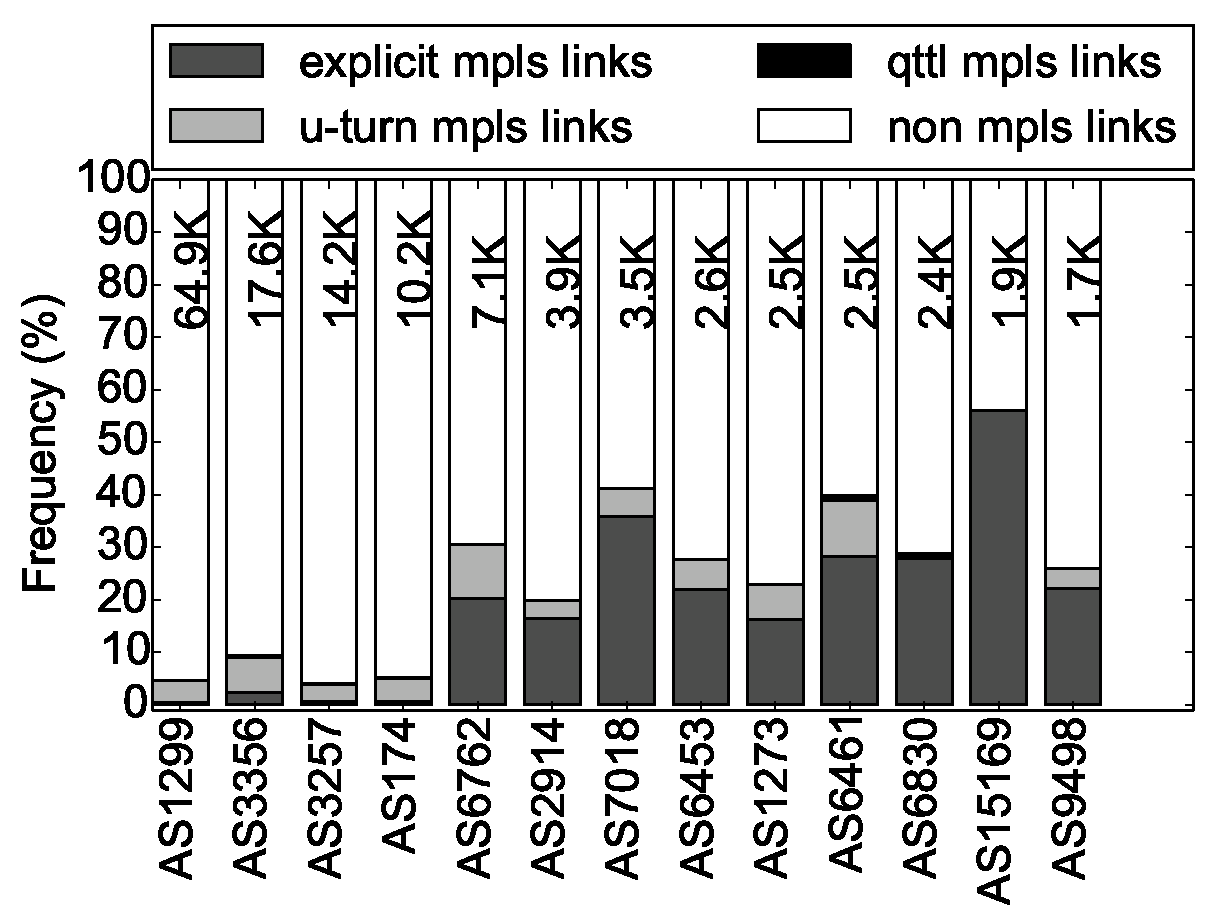
\includegraphics[width=8cm]{TOP_AS}
  \end{center}
  \caption{Top of ASes with most links discovered} On top four ASes
  prevails \textit{u-turn mpls links}. On the rest of ASes prevails \textit{qttl
  mpls links.}
  \label{top_as}
\end{figure}

%Figura u-turn
\begin{figure*}[!htb]
  \begin{center}
    \subfigure[AS1299  Teliasonera AB , $C_{\max}=21$, $\text{Degree}_{\max}=2781$, $\vert V_{r
    \backslash lsr} \vert=4128$, $\vert E_{r \backslash lsr} \vert=24865$ ]{\label{fig_cluster_mpls_1299}
      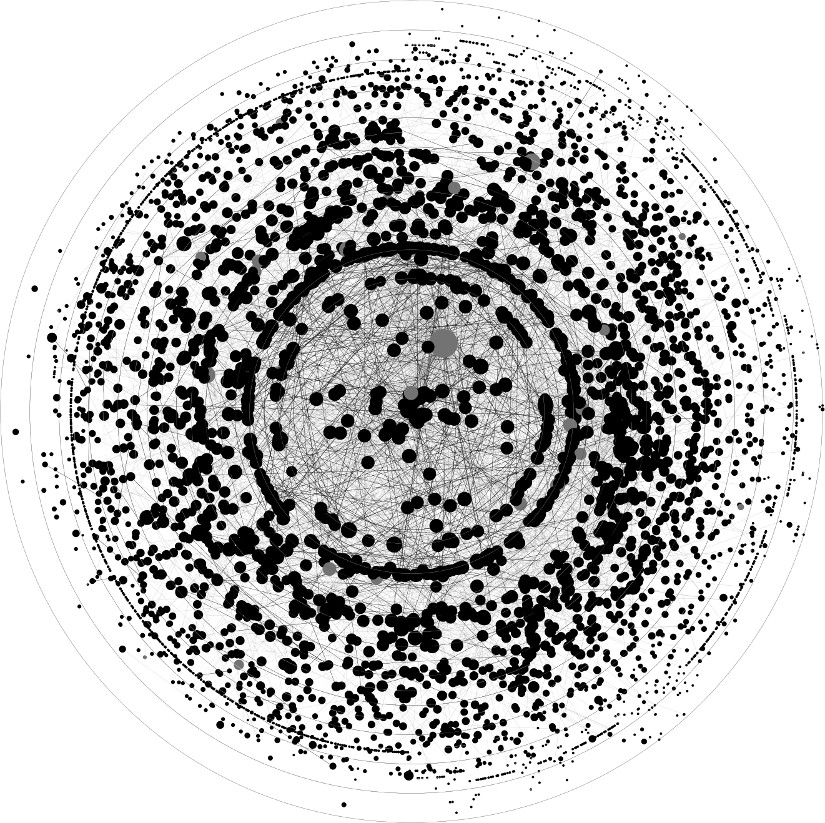
\includegraphics[width=2in]{1299}}
\hfill
    \subfigure[AS174 Cogent Communication, $C_{\max}=8$, $\text{Degree}_{\max}=751$,$\vert V_{r
    \backslash lsr} \vert=4421$, $\vert E_{r \backslash lsr} \vert=8611$]{\label{fig_cluster_mpls_174}
      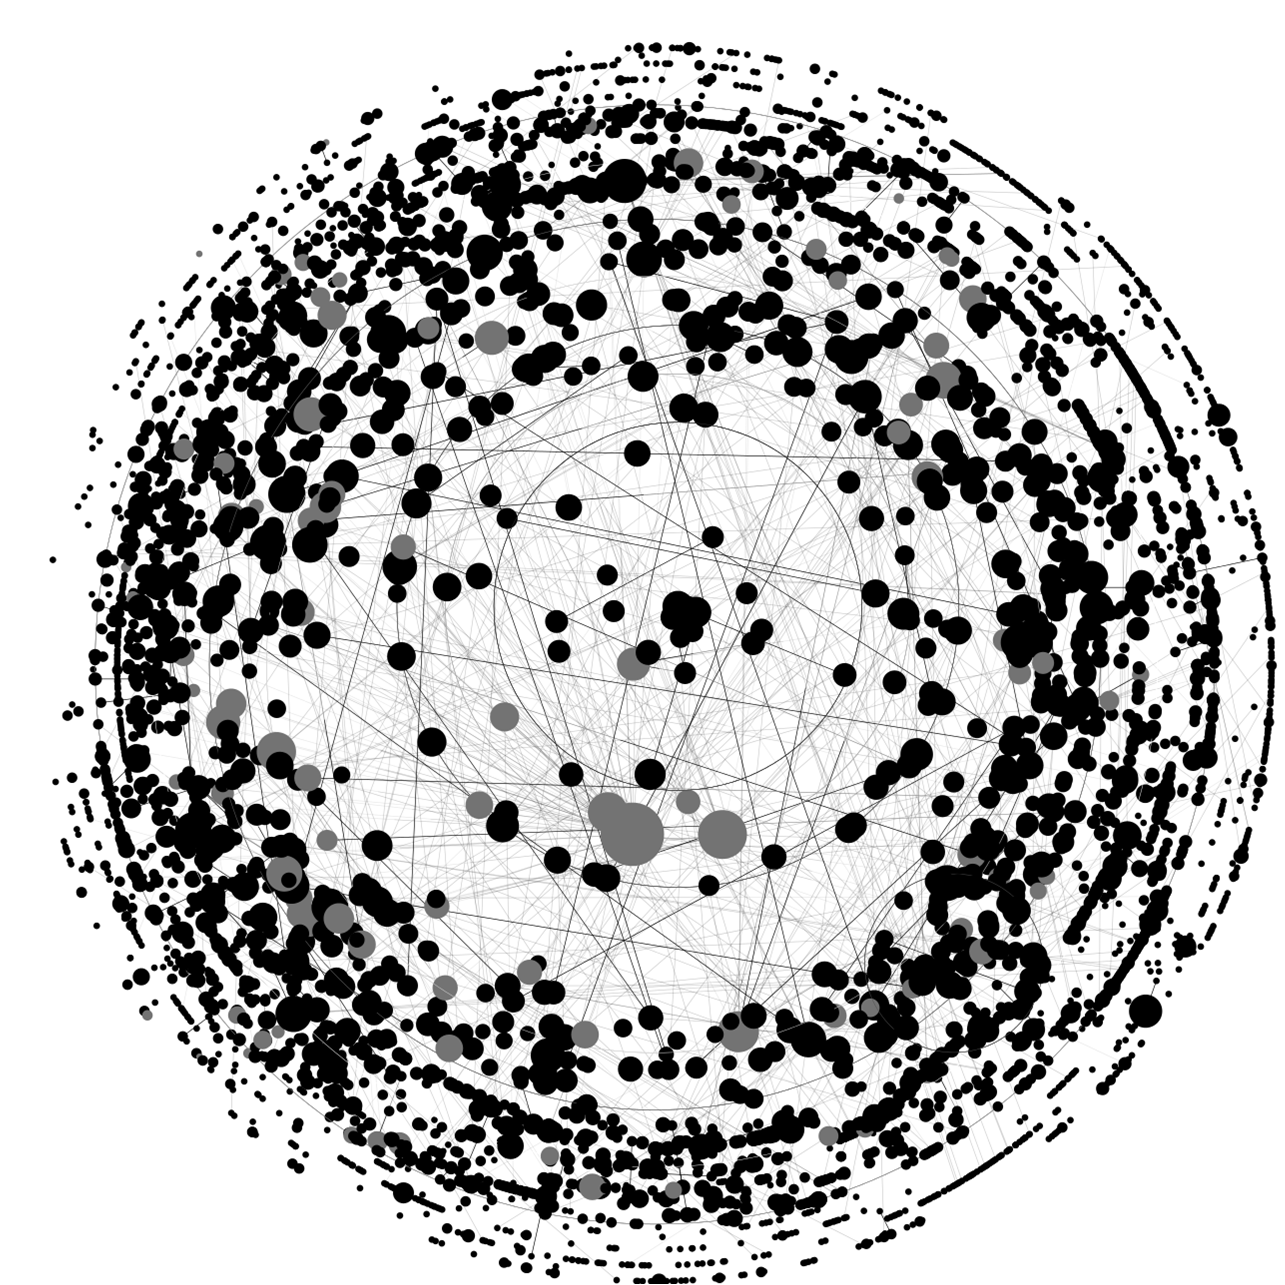
\includegraphics[width=2in]{174}}
\hfill
    \subfigure[AS6762 Telecom Italia, $C_{\max}=10$, $\text{Degree}_{\max}=564$,$\vert V_{r
    \backslash lsr} \vert=750$, $\vert E_{r \backslash lsr} \vert=1504$]{\label{fig_cluster_mpls_6762}
      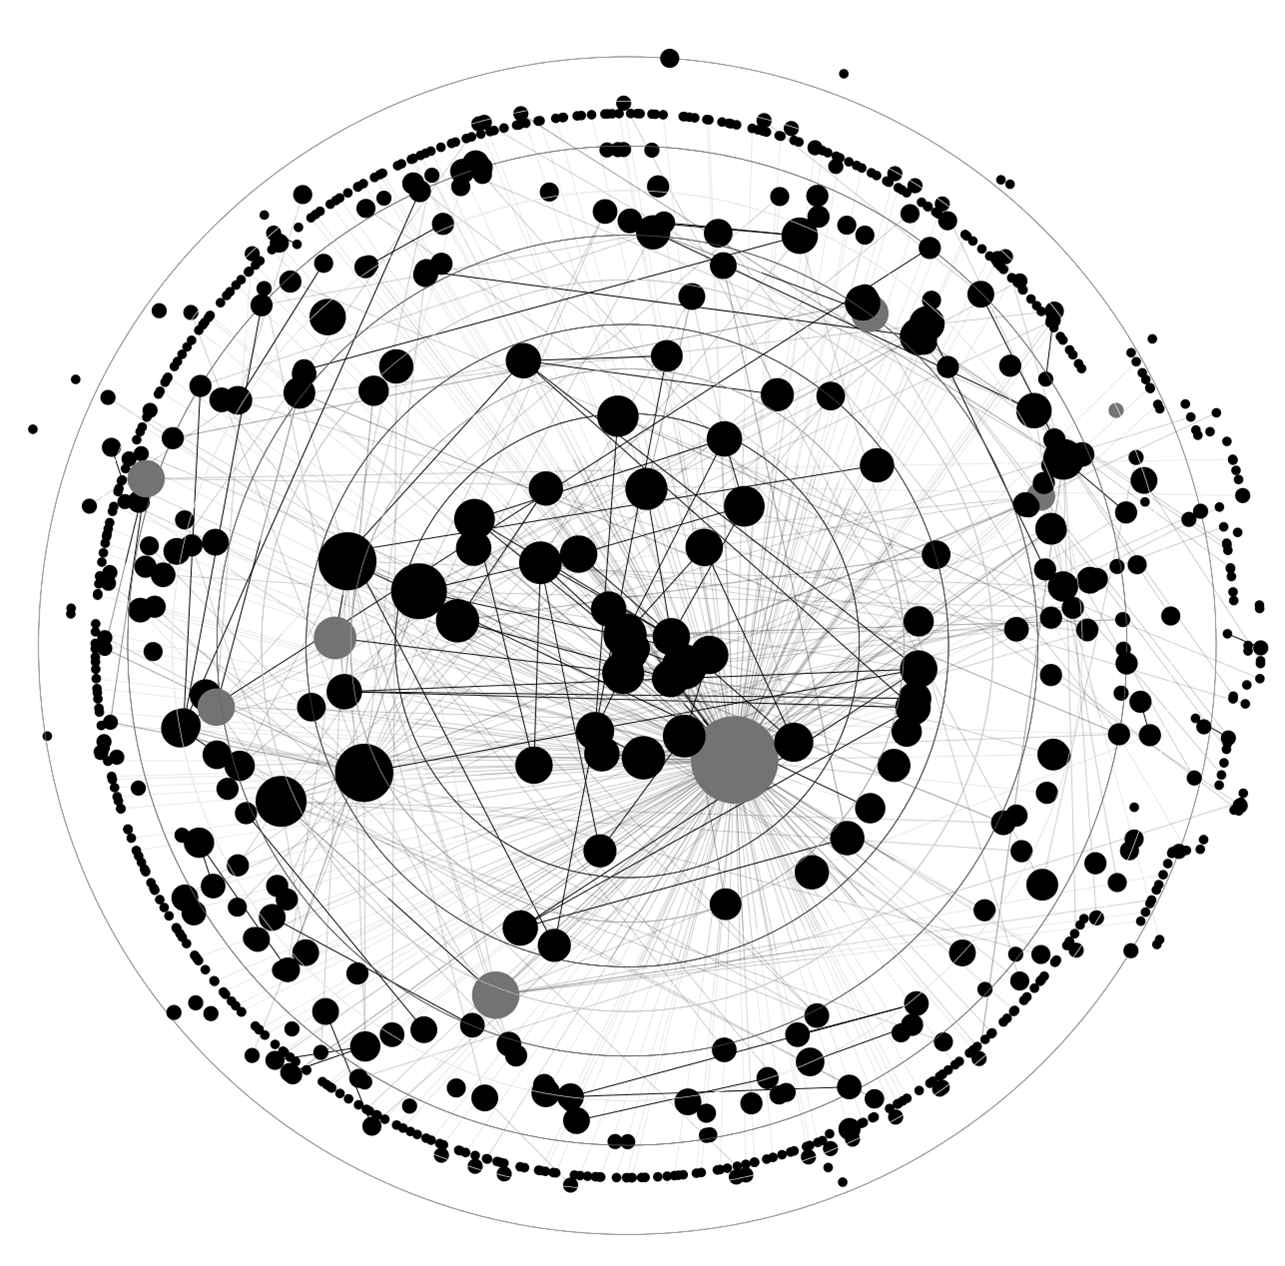
\includegraphics[width=2in]{6762}}
\hfill
    \subfigure[AS2914 NTT America Inc., $C_{\max}=4$, $\text{Degree}_{\max}=1019$,$\vert V_{r
    \backslash lsr} \vert=1807$, $\vert E_{r \backslash lsr} \vert=2360$]{\label{fig_cluster_mpls_2914}
      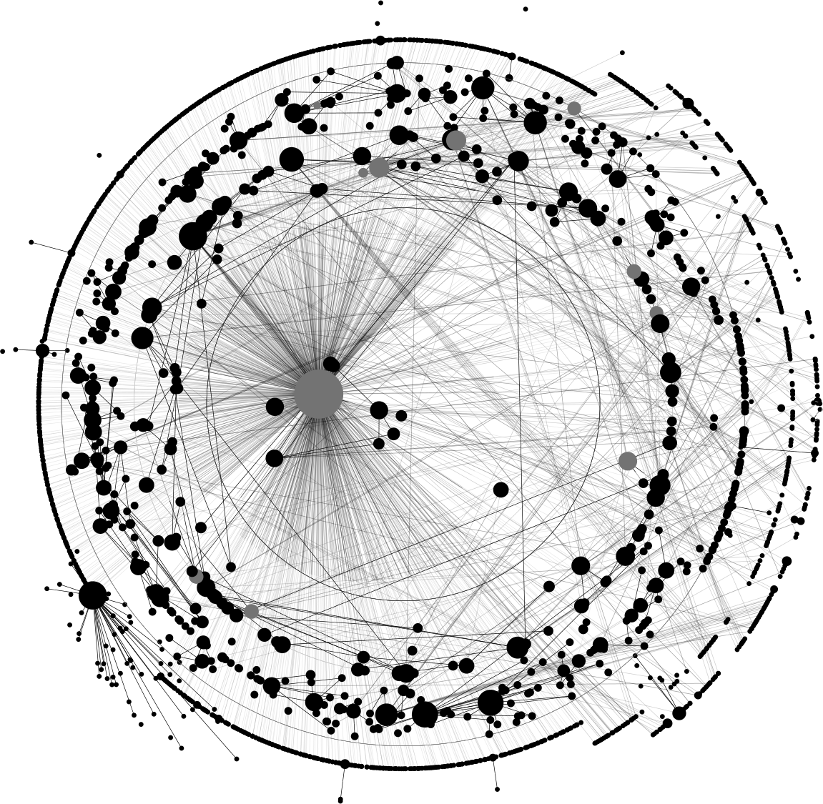
\includegraphics[width=2in]{2914}}
\hfil
    \subfigure[ AS7018 AT\&T, $C_{\max}=3$, $\text{Degree}_{\max}=745$, $\vert V_{r
    \backslash lsr} \vert=1306$, $\vert E_{r \backslash lsr} \vert=1441$]{\label{fig_cluster_mpls_7018}
      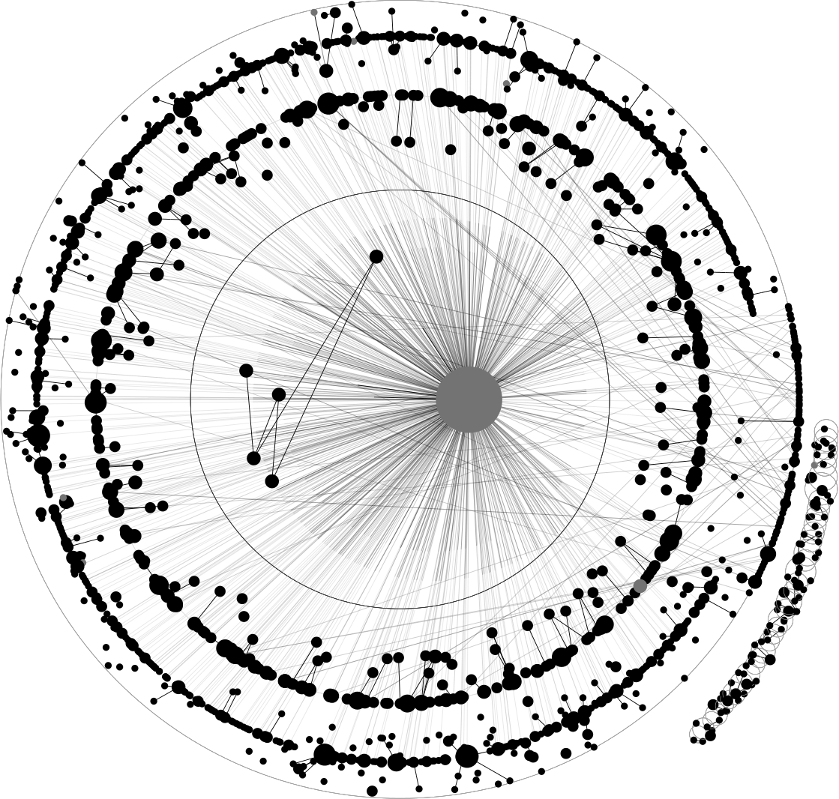
\includegraphics[width=2in]{7018}}
\hfil
    \subfigure[ AS1273 Cable and Wireless Worldwide plc, $C_{\max}=3$, $\text{Degree}_{\max}=806$, $\vert V_{r \backslash lsr} \vert=1127$, $\vert E_{r \backslash lsr} \vert=1215$]{\label{fig_cluster_mpls_1273}
      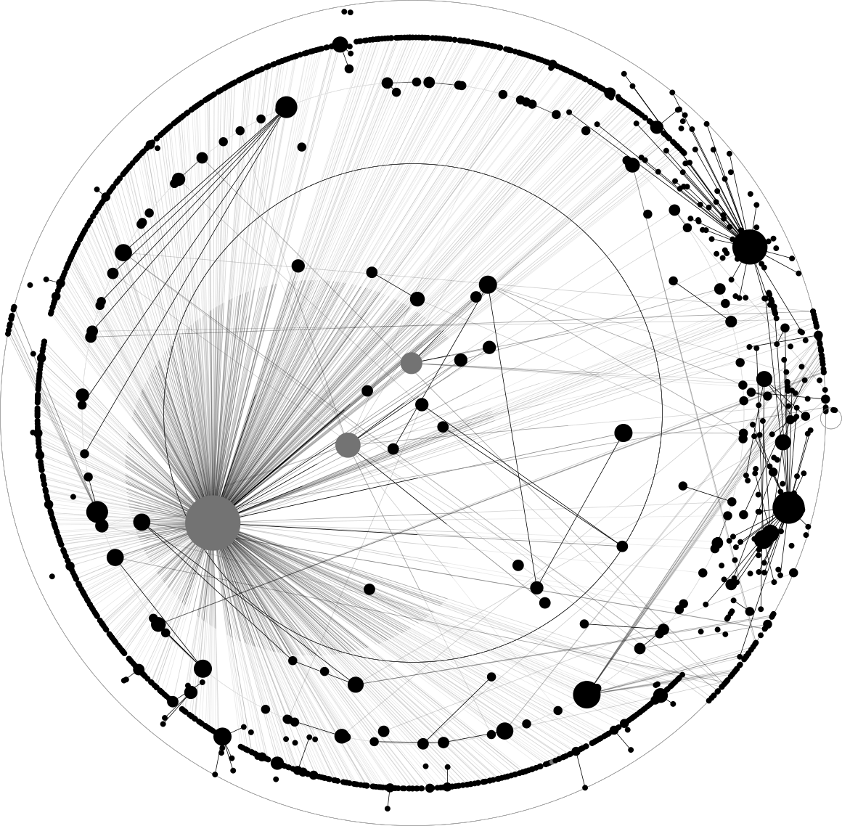
\includegraphics[width=2in]{1273}}
  \end{center}
  \caption{$k$-core visualization of MPLS cluster interconnection Graph
  $G_{r\backslash lsr}(as)$. On the top the ASes show \textit{MPLS clusters}
  spread out around the shell index of the decomposition. On the bottom the ASes
  show \textit{MPLS clusters} well defined and located on the top core
  $C_{\max}$.}
  \label{fig_cluster_mpls}
\end{figure*}
\section{Conclusion}\label{ccl}
%%%%%%%%%%%%%%%%%%%%
 
\section*{Acknowledgments}\label{ack}
%%%%%%%%%%%%%%%%%%%%%%%%%%
This work is partially funded by the European Commission funded mPlane
ICT-318627 project.


{\small
 \bibliographystyle{IEEEtran}
 \bibliography{Bibliography}
}

\end{document}
